% Options for packages loaded elsewhere
\PassOptionsToPackage{unicode}{hyperref}
\PassOptionsToPackage{hyphens}{url}
\documentclass[
  10pt,
]{article}
\usepackage[table]{xcolor}
\usepackage{amsmath,amssymb}
\setcounter{secnumdepth}{5}
\usepackage{iftex}
\ifPDFTeX
  \usepackage[T1]{fontenc}
  \usepackage[utf8]{inputenc}
  \usepackage{textcomp} % provide euro and other symbols
\else % if luatex or xetex
  \usepackage{unicode-math} % this also loads fontspec
  \defaultfontfeatures{Scale=MatchLowercase}
  \defaultfontfeatures[\rmfamily]{Ligatures=TeX,Scale=1}
\fi
\usepackage{lmodern}
\ifPDFTeX\else
  % xetex/luatex font selection
\fi
% Use upquote if available, for straight quotes in verbatim environments
\IfFileExists{upquote.sty}{\usepackage{upquote}}{}
\IfFileExists{microtype.sty}{% use microtype if available
  \usepackage[]{microtype}
  \UseMicrotypeSet[protrusion]{basicmath} % disable protrusion for tt fonts
}{}
\makeatletter
\@ifundefined{KOMAClassName}{% if non-KOMA class
  \IfFileExists{parskip.sty}{%
    \usepackage{parskip}
  }{% else
    \setlength{\parindent}{0pt}
    \setlength{\parskip}{6pt plus 2pt minus 1pt}}
}{% if KOMA class
  \KOMAoptions{parskip=half}}
\makeatother
\usepackage{longtable,booktabs,array}
\newcounter{none} % for unnumbered tables
\usepackage{calc} % for calculating minipage widths
% Correct order of tables after \paragraph or \subparagraph
\usepackage{etoolbox}
\makeatletter
\patchcmd\longtable{\par}{\if@noskipsec\mbox{}\fi\par}{}{}
\makeatother
% Allow footnotes in longtable head/foot
\IfFileExists{footnotehyper.sty}{\usepackage{footnotehyper}}{\usepackage{footnote}}
\makesavenoteenv{longtable}
\usepackage{graphicx}
\makeatletter
\newsavebox\pandoc@box
\newcommand*\pandocbounded[1]{% scales image to fit in text height/width
  \sbox\pandoc@box{#1}%
  \Gscale@div\@tempa{\textheight}{\dimexpr\ht\pandoc@box+\dp\pandoc@box\relax}%
  \Gscale@div\@tempb{\linewidth}{\wd\pandoc@box}%
  \ifdim\@tempb\p@<\@tempa\p@\let\@tempa\@tempb\fi% select the smaller of both
  \ifdim\@tempa\p@<\p@\scalebox{\@tempa}{\usebox\pandoc@box}%
  \else\usebox{\pandoc@box}%
  \fi%
}
% Set default figure placement to htbp
\def\fps@figure{htbp}
\makeatother
\setlength{\emergencystretch}{3em} % prevent overfull lines
\providecommand{\tightlist}{%
  \setlength{\itemsep}{0pt}\setlength{\parskip}{0pt}}
\usepackage{rxp_report}
\usepackage{fancyhdr}
\usepackage{draftwatermark}
\SetWatermarkLightness{0.88}
\usepackage{etoc}
\usepackage{bookmark}
\IfFileExists{xurl.sty}{\usepackage{xurl}}{} % add URL line breaks if available
\urlstyle{same}
\hypersetup{
  hidelinks,
  pdfauthor={Mehmet Yunt},
  pdftitle={Task Grouping Analysis},
  pdfcreator={LaTeX via pandoc}}
\fancypagestyle{report}{%
  \fancyhf{}%
  \fancyfoot[L]{\footnotesize Task Grouping Analysis}%
  \fancyfoot[C]{\thepage}%
  \fancyfoot[R]{\footnotesize Mehmet Yunt}%
  \renewcommand{\headrulewidth}{0pt}%
  \renewcommand{\footrulewidth}{0pt}%
}
\pagestyle{report}

\title{Task Grouping Analysis}
\author{Mehmet Yunt}
\date{\today}

\begin{document}
\thispagestyle{plain}
\noindent{\Large\bfseries\color{red}DRAFT}\par\smallskip
\noindent{\large\bfseries\color{reportnavy}Task Grouping Analysis}\par
\noindent\textbf{Author:} Mehmet Yunt\par
\noindent\textbf{Date:} \today\par\medskip
\section{Executive Summary}\label{abstract}
A task scheduling system could place similar DUR tasks in succession; reducing efficiency loss due to context switching.

Using historical RxBuddy DUR tasks from 2026-01-02 to 2026-08-01, it is estimated that the duration of a DUR task can be 3.4\%
less if it follows a DUR of the same cohort immediately than in the case it is preceded by a DUR of different cohort. See section
\ref{modeling-dur-processing-time} for more details.

The annualized potential savings in pharmacist labor value is estimated to be of the range \$80,000--\$88,000 per year. See section
\ref{estimating-potential-cost-savings} obtained by applying the 3.4\% reduction to successful DUR tasks that are not already preceded by DURs of the same cohort
assuming maximum scheduling flexibility.

We note that the results are based on an observational study and not a randomized controlled experiment where the effects of
confounding factors could be randomized away. Therefore, the results should be taken with a grain of salt.

\section{Appendix}\label{appendix}
\etocsettocdepth{subsubsection}
\etocsettocstyle{\noindent\textcolor{reportnavy}{\textbf{Appendix contents}}\par\smallskip}{\par}
\localtableofcontents
\subsection{Reproducing the Numerical Results}
The code to reproduce all the results is in \ref{ref:analysis-repository}. Follow the instructions in the HOWTO.md file to generate the figures, models and analyses.
You will need to clone the repository to run the code. The code uses make and python.
In addition you need to have access to a Snowflake role that has access to the following tables:
\begin{verbatim}
 EDLDB.PET_HEALTH_ANALYTICS_SANDBOX.FCT__TASKS_LIFECYCLE
 EDLDB.BT_HCA_HCDM.RXP_RX_USAGE_ACTIONS
 CHEWYBI.CUSTOMER_PETPROFILES
 EDLDB.PDM.PRODUCT
 EDLDB.BT_HCA_HCDM.RXP_PRESCRIPTIONS
\end{verbatim}
and the pet health analytics sandbox in the dev environment;
\begin{verbatim}
 EDLDB_DEV.PET_HEALTH_ANALYTICS_SANDBOX
\end{verbatim}
to generate transient tables.

\subsection{Cohort Definitions}
This section is verbatim reproduced from the conversation with JD Wright to provide
background on the history of cohorts and their rationale.

\textbf{Cohort 1}: Boxed parasiticides. This was the best starting point
because it represents roughly 40\% of total DUR volume and the
majority of the initial digital volume, while the clinical rules are
relatively standardized and label-driven. The primary checks are
species, weight range, monthly directions, days\textquotesingle{}
supply, duplicate parasite coverage, and known contraindications. This
gave us a high-volume population with relatively low variability for
validating the core RxBuddy and DUR Copilot experience.

\textbf{Cohort 2}: Non-controlled, non-boxed medications. This represents
roughly 29\% of total DUR volume and materially expands coverage, but
the clinical review is more complex. These medications require
generalized dosing evaluation, including strength, dose, frequency,
route, indication, species appropriateness, duplicate therapy,
contraindications, and potential interactions. We separated this
cohort so those broader AI checks could be validated without also
introducing compounding or controlled-substance requirements at the
same time.

\textbf{Cohort 3}: Non-controlled compounded medications. This is a smaller
segment at roughly 4.4\% of DUR volume, but it has distinct clinical
and compliance requirements. Compounds require a documented
compounding reason, formulation-specific directions, and validation
that the prescribed days\textquotesingle{} supply does not exceed the
product\textquotesingle s beyond-use date. BUD rules vary by dosage
form, storage conditions, formulation, and stability-study results.
Keeping compounds separate allowed us to test these specialized
workflows and manage their impact on pharmacist throughput
independently.

\textbf{Cohort 4}: Gabapentin and the high-scrutiny regulatory workflow. This
represents roughly 1.1\% of DUR volume. The implemented Phase 4 scope
focused on uncontrolled gabapentin rather than the full
controlled-substance population, but it was separated because it
introduces site eligibility, pharmacist skill gating, regulatory
indicators, mixed-order handling, and state-specific scrutiny. It also
gave us a contained way to validate infrastructure that will be needed
for broader controlled-substance support later.

\subsection{Motivating Example for Building a Detailed Model}
In this section, two task sequences from the same user are examined.

Both sequences have MC3 \texttt{Parasiticide} and approval channel
\texttt{PH}. All start times have UTC offset \texttt{+0000} and
\texttt{.000} milliseconds; blank updated fields mean no fields were
updated.

Sequence A: pet \texttt{Dog}, initiation channel \texttt{AUTOSHIP}.

{\def\LTcaptype{none} % do not increment counter
\begin{longtable}[]{@{}rrrll@{}}
\toprule\noalign{}
Order & Part number & Duration (s) & Start time (UTC) & Updated
fields \\
\midrule\noalign{}
\endhead
\bottomrule\noalign{}
\endlastfoot
1 & 146066 & 40 & 2026-04-30 06:42:54 & \\
2 & 152702 & 27 & 2026-04-30 06:43:36 & directions \\
3 & 146391 & 40 & 2026-04-30 06:44:06 & \\
4 & 151583 & 7 & 2026-04-30 06:44:48 & \\
5 & 146138 & 7 & 2026-04-30 06:44:56 & \\
6 & 146142 & 43 & 2026-04-30 06:45:05 & directions \\
7 & 146142 & 35 & 2026-04-30 06:45:49 & directions \\
8 & 146064 & 39 & 2026-04-30 06:46:26 & directions \\
9 & 146167 & 12 & 2026-04-30 06:47:07 & \\
10 & 146322 & 9 & 2026-04-30 06:47:21 & directions \\
11 & 146167 & 97 & 2026-04-30 06:47:32 & directions \\
12 & 146050 & 6 & 2026-04-30 06:49:11 & \\
13 & 146387 & 54 & 2026-04-30 06:49:19 & \\
\end{longtable}
}

Sequence B: pet \texttt{Cat}, initiation channel \texttt{OMS}.

{\def\LTcaptype{none} % do not increment counter
\begin{longtable}[]{@{}rrrll@{}}
\toprule\noalign{}
Order & Part number & Duration (s) & Start time (UTC) & Updated
fields \\
\midrule\noalign{}
\endhead
\bottomrule\noalign{}
\endlastfoot
1 & 158995 & 11 & 2026-07-15 02:17:23 & \\
2 & 158995 & 35 & 2026-07-15 02:17:36 & \\
3 & 158995 & 3 & 2026-07-15 02:18:13 & \\
4 & 158995 & 13 & 2026-07-15 02:18:17 & \\
5 & 158995 & 13 & 2026-07-15 02:18:31 & \\
6 & 158995 & 6 & 2026-07-15 02:18:46 & \\
7 & 158995 & 16 & 2026-07-15 02:18:53 & \\
8 & 158995 & 13 & 2026-07-15 02:19:11 & \\
9 & 158995 & 6 & 2026-07-15 02:19:25 & \\
10 & 158995 & 50 & 2026-07-15 02:19:32 & \\
11 & 158998 & 11 & 2026-07-15 02:20:23 & \\
12 & 158998 & 29 & 2026-07-15 02:20:36 & \\
\end{longtable}
}

The second sequence demonstrates substantial inherent variability in DUR
times.

\subsection{Some Factors of DUR Duration}
\subsubsection{Pharmacist Performance}
Pharmacists vary in their speed to process DURs.

\begin{center}
\pandocbounded{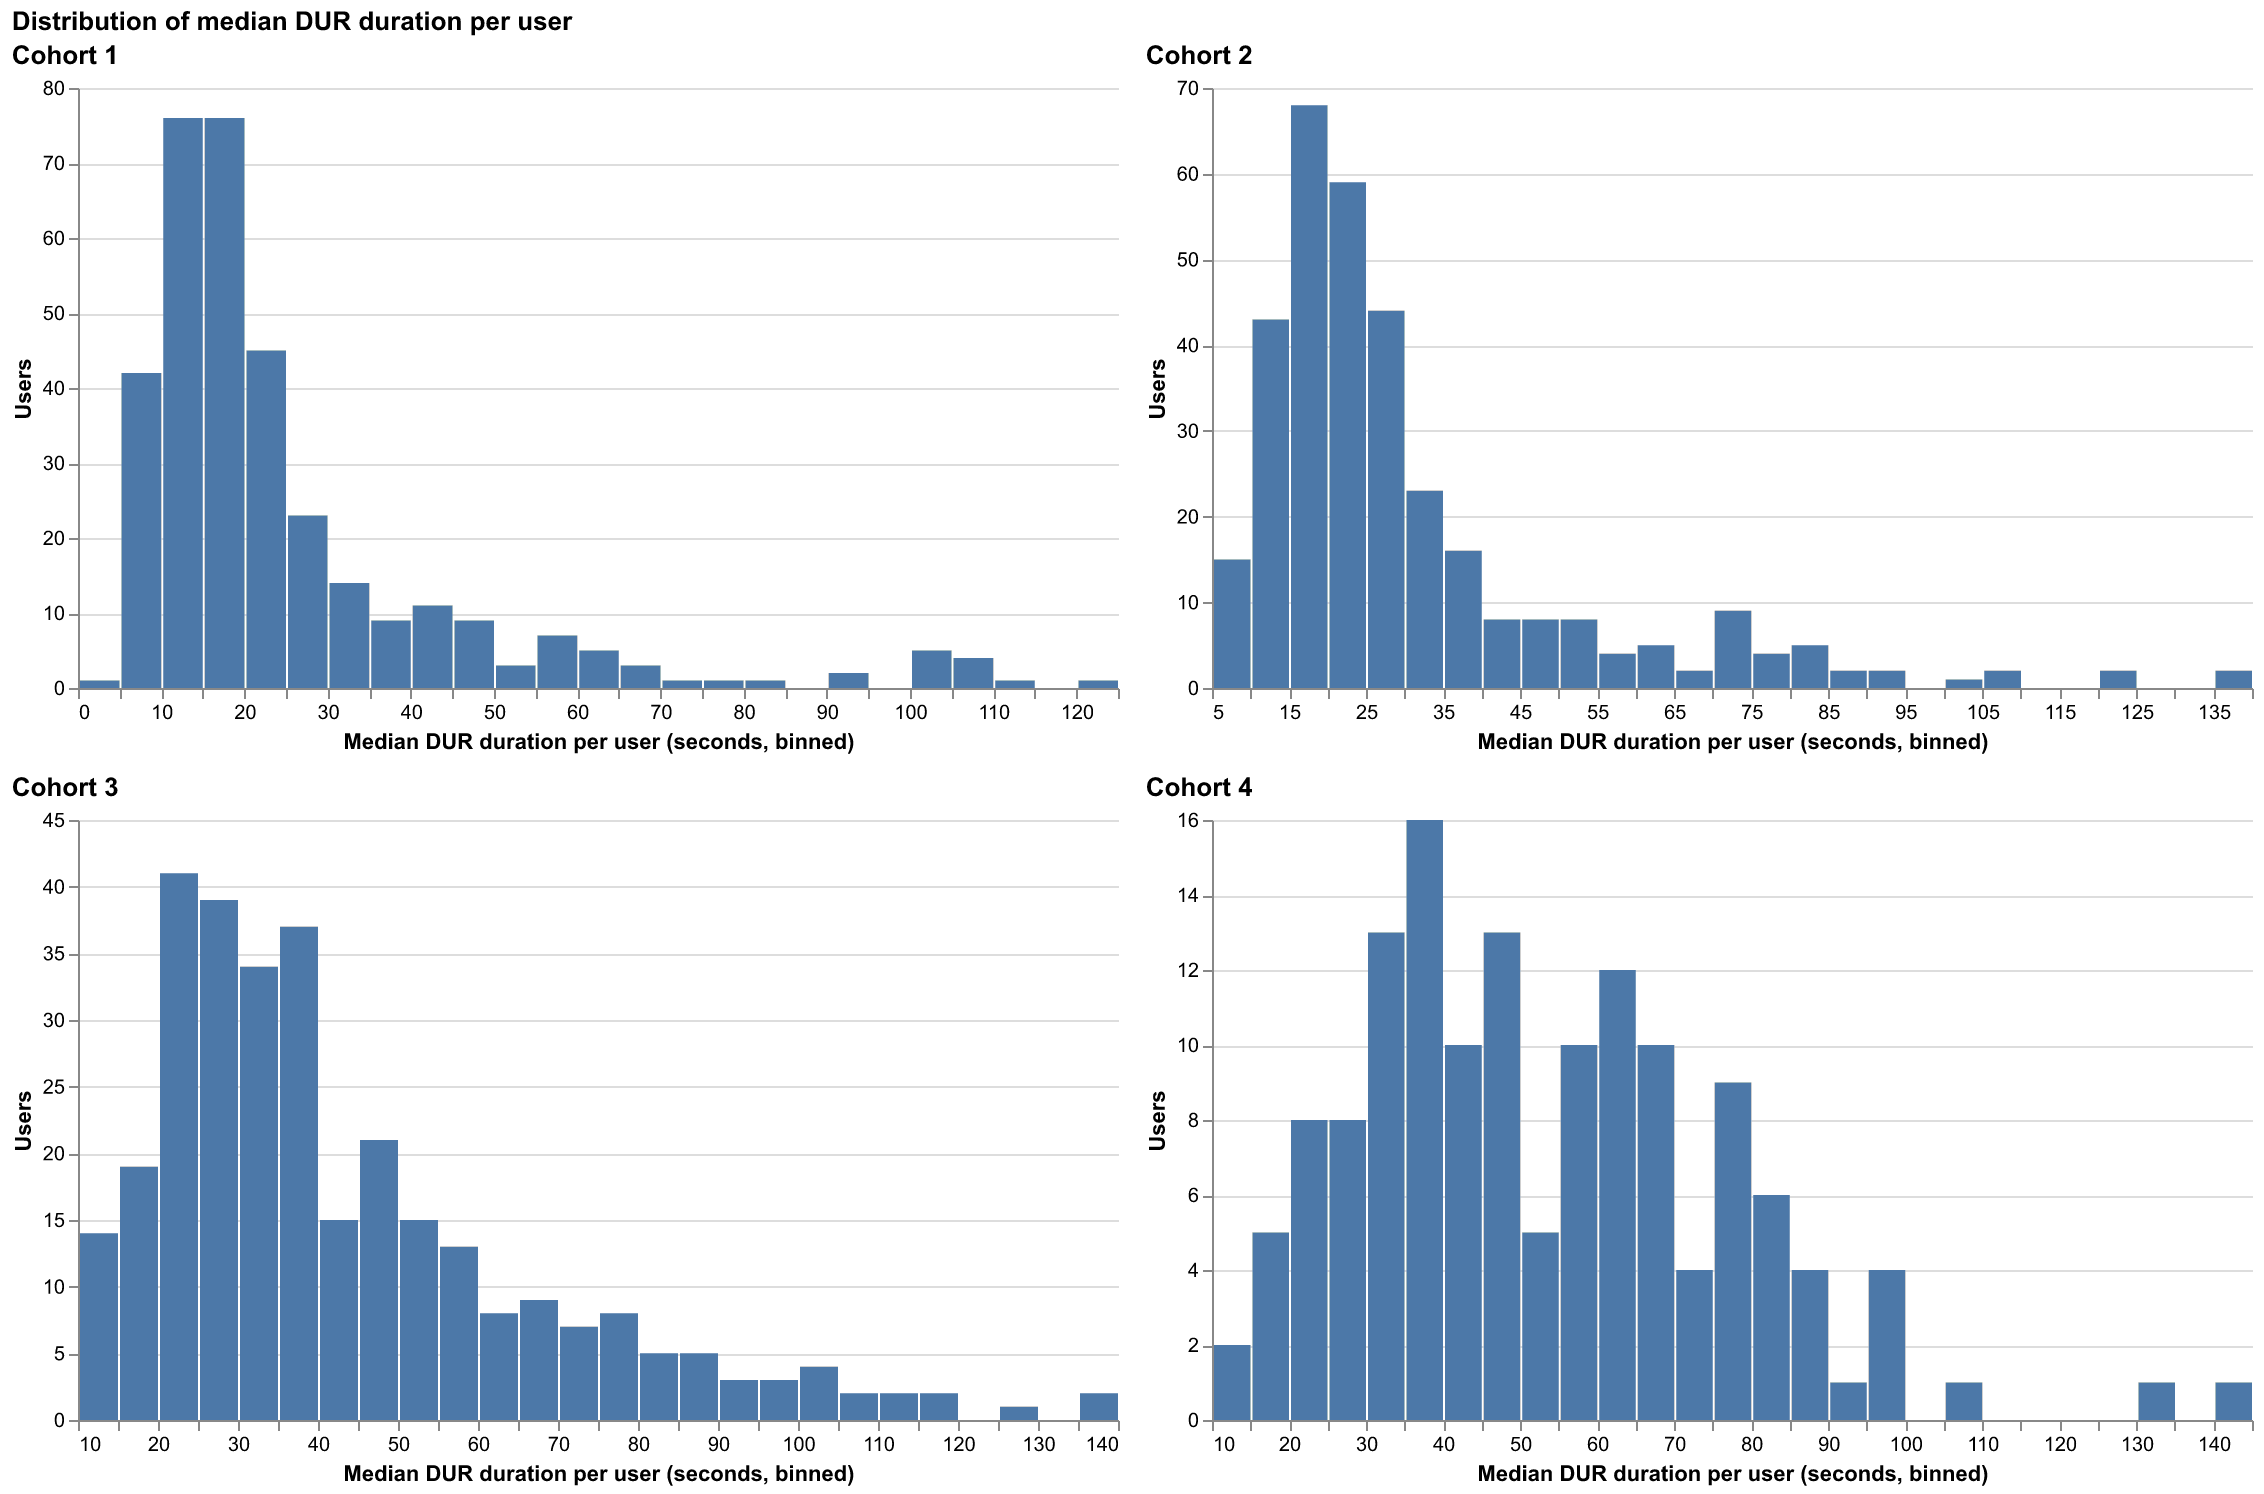
\includegraphics[keepaspectratio,alt={Distribution of median DUR duration per user by cohort}]{outputs/charts/user-performance-analysis/user-median-dur-duration-distributions.png}}
\end{center}

If a pharmacist is fast in handling a cohort 1 DUR, highly likely he/she is also fast handling other cohort DURs.

\begin{center}
\pandocbounded{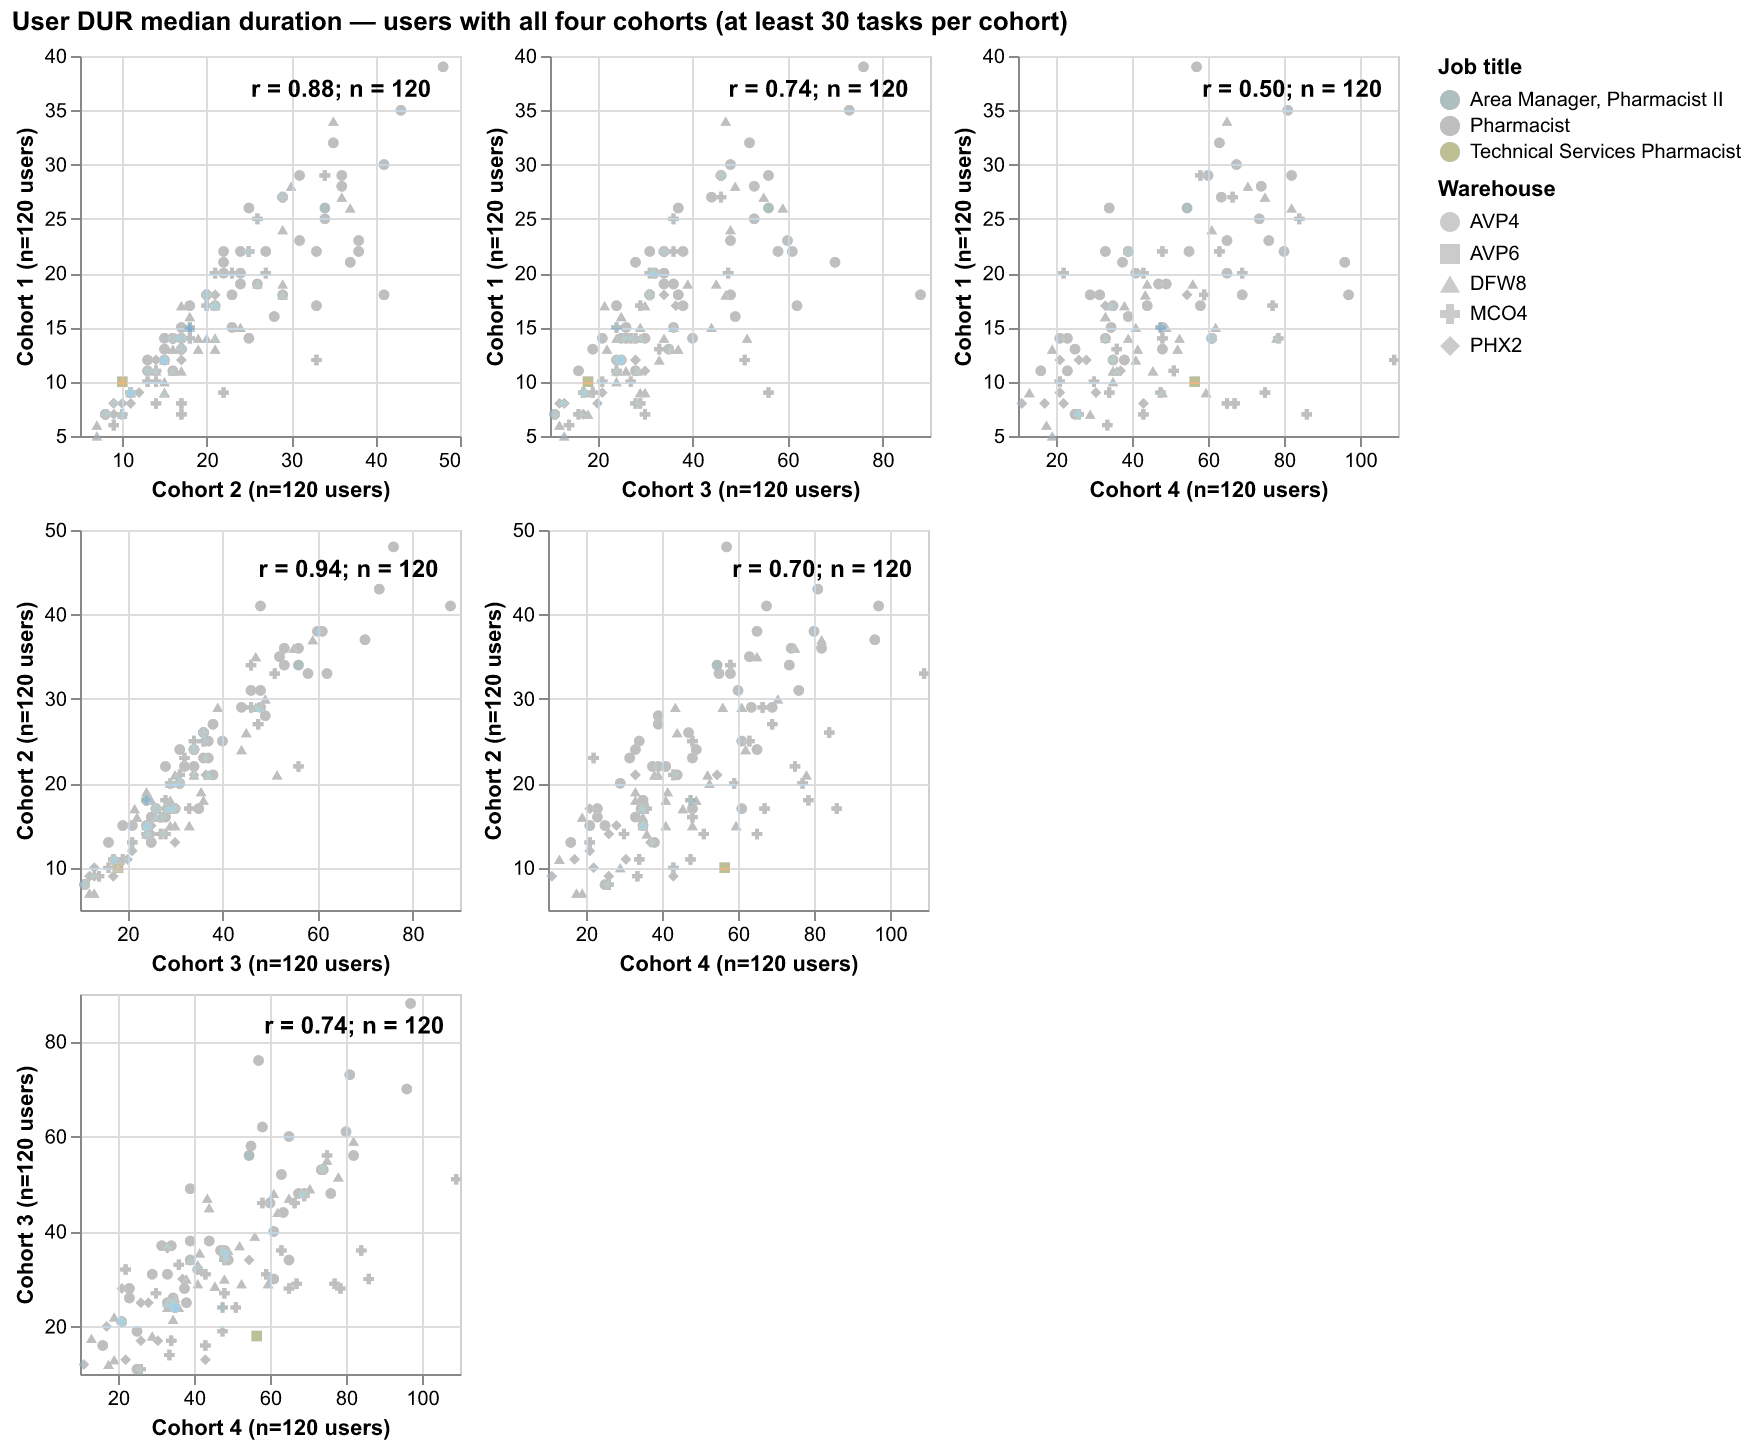
\includegraphics[keepaspectratio,alt={Scatter matrix of user median DUR duration across all four cohorts}]{outputs/charts/user-performance-analysis/user-performance-median-all-cohorts-scatter-matrix.png}}
\end{center}

\subsection{One-Sided Paired Comparison Test} \label{cohort-user-one-sided-comparison}
In this section, a paired-test is carried out to determine if a task
preceded by the same task is executed faster.  The tests show that for
cohort 1,2,3 there is a non-zero improvement but for cohort 4, the
test cannot reject that there is no improvement.

The method does not try to test for confounders \ref{ref:confounding}  which are possible factors affecting both the decision of scheduling one task after another and the output which is duration. In this study, we try to account for the user and the cohort, but we are not able to control for day of the week, pet or part number which might be in the set of confounders. Confounders can change the analysis result significantly.
A similar approach in \ref{ref:grouping-similar-work} points out that there is statistical reason to believe that controlling for cohort and user still may not eliminate the effect of confounders.

\subsubsection{Purpose and method}
This analysis compares Same Cohort and Different Cohort DUR work time within
users, separately for Cohorts 1--4. Task durations are first averaged within
each user, cohort, and allocation pattern. Only users with both allocation
patterns in the same cohort are retained, so the comparison is paired by user.

The paired test is a one-sided paired $t$-test. The null hypothesis is that
Same Cohort is not faster than Different Cohort
($\text{Same Cohort}-\text{Different Cohort}\geq 0$); the alternative is
that this difference is less than zero, with $\alpha=0.05$. The density
plots in Figures~\ref{fig:cohort-user-one-sided-1}--\ref{fig:cohort-user-one-sided-4}
show the two distributions of user-level means on a base-10 logarithmic
horizontal axis.

The 95\% two-sided confidence intervals for each allocation-pattern mean and
the paired mean difference use Student's $t$ distribution and the matched
users as the units of analysis. The one-sided 95\% upper bounds correspond to
the directional paired tests.

The source query keeps transitions on or after 2026-08-01, DUR tasks with
final status \texttt{CLOSED}, non-null user and start time, work time between
0.01 and 5 minutes, and known item cohorts. Rows without a previous cohort
are excluded.

\subsubsection{User-level work-time densities}
\begin{center}
\begin{minipage}{\linewidth}
\centering
\begin{minipage}[t]{0.49\linewidth}
\vspace{0pt}\centering
\fbox{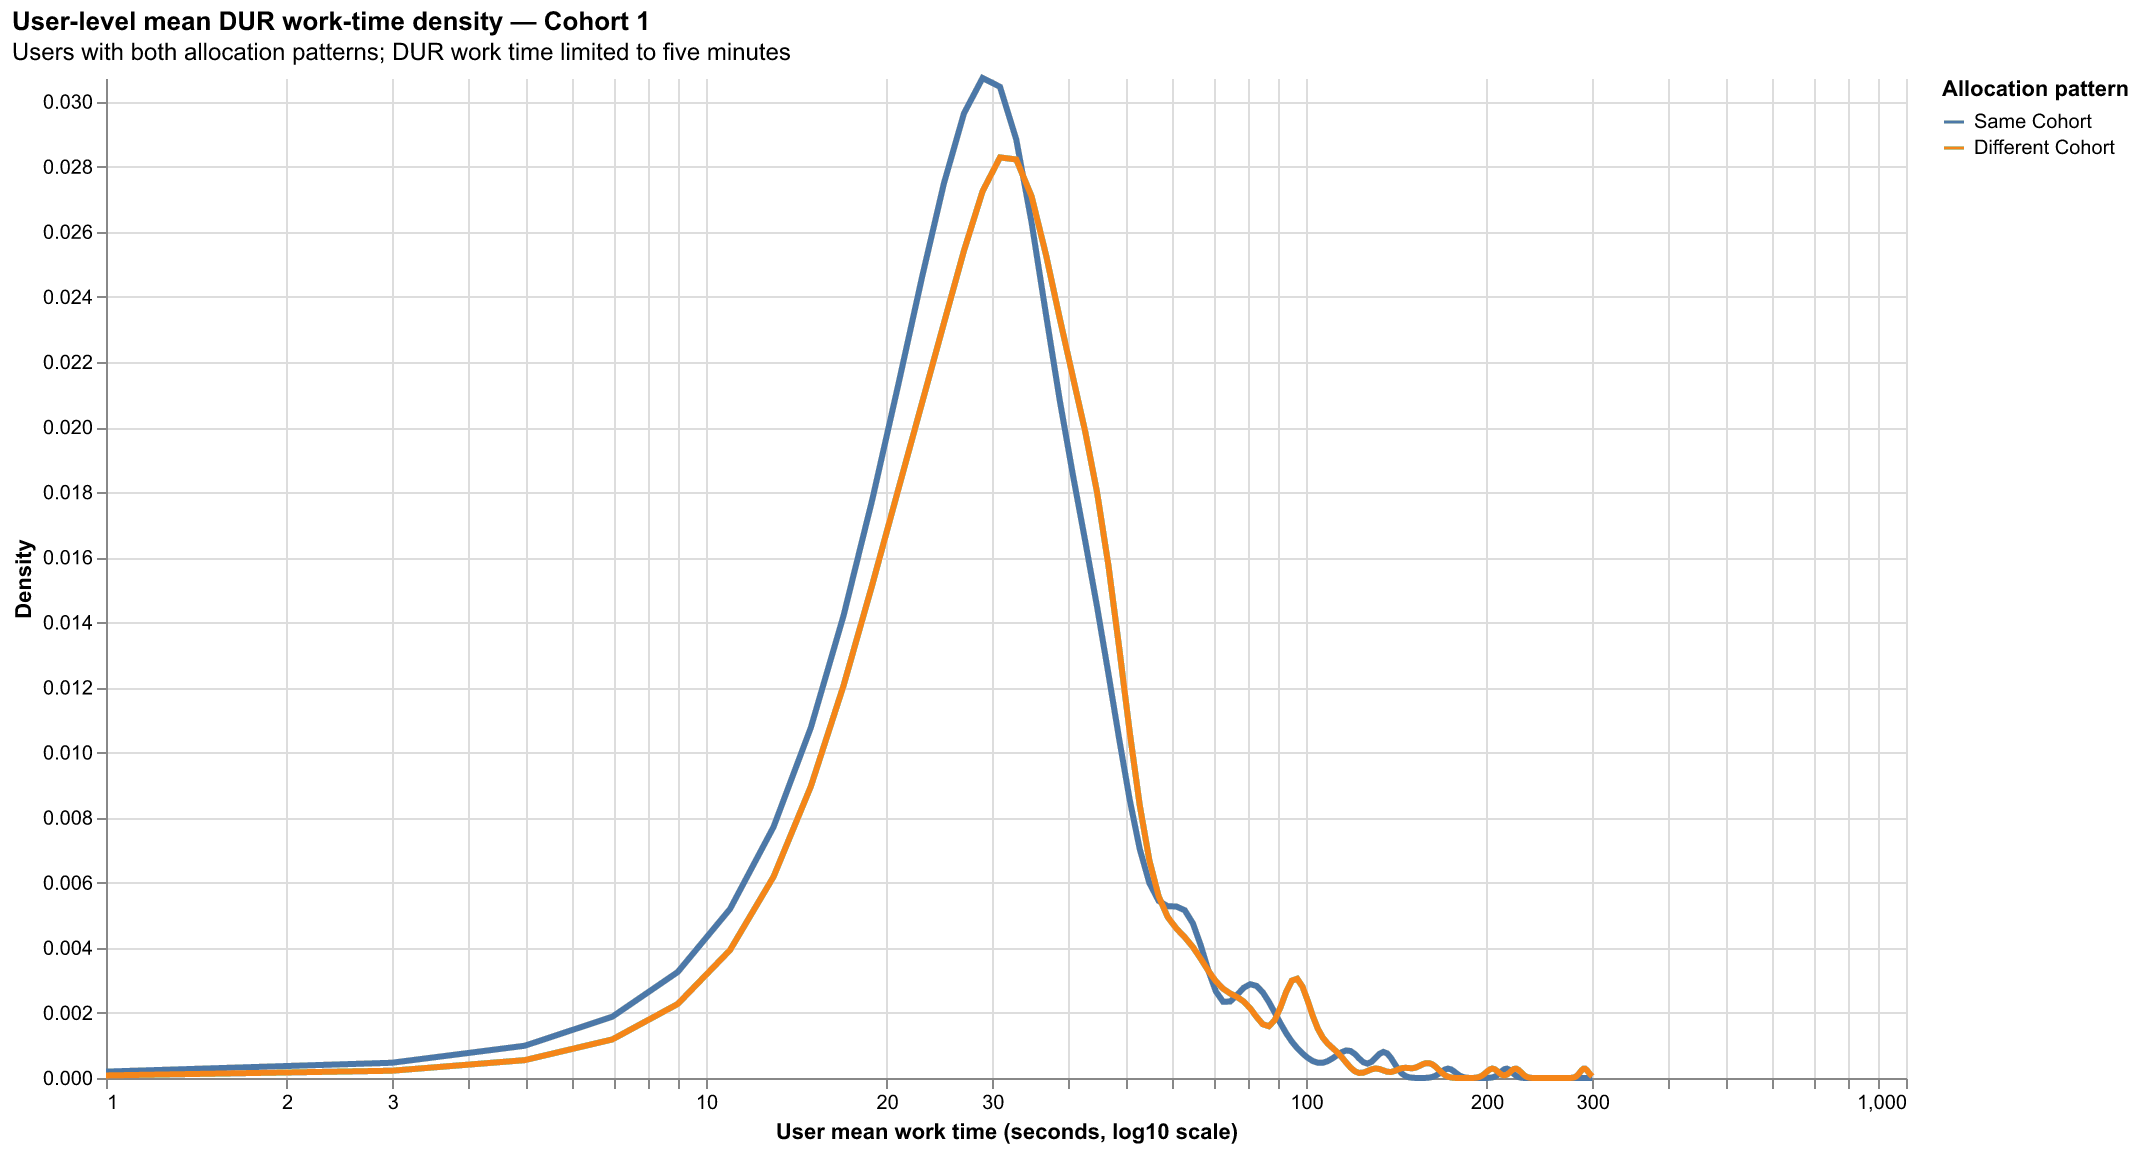
\includegraphics[width=\dimexpr\linewidth-2\fboxsep-2\fboxrule\relax,keepaspectratio,alt={User-level work-time density for Cohort 1}]{outputs/charts/stats-comparison-user/stats-comparison-user-cohort-1.png}}
\captionof{figure}{User-level work-time density, Cohort 1.}\label{fig:cohort-user-one-sided-1}
\end{minipage}\hfill
\begin{minipage}[t]{0.49\linewidth}
\vspace{0pt}\centering
\fbox{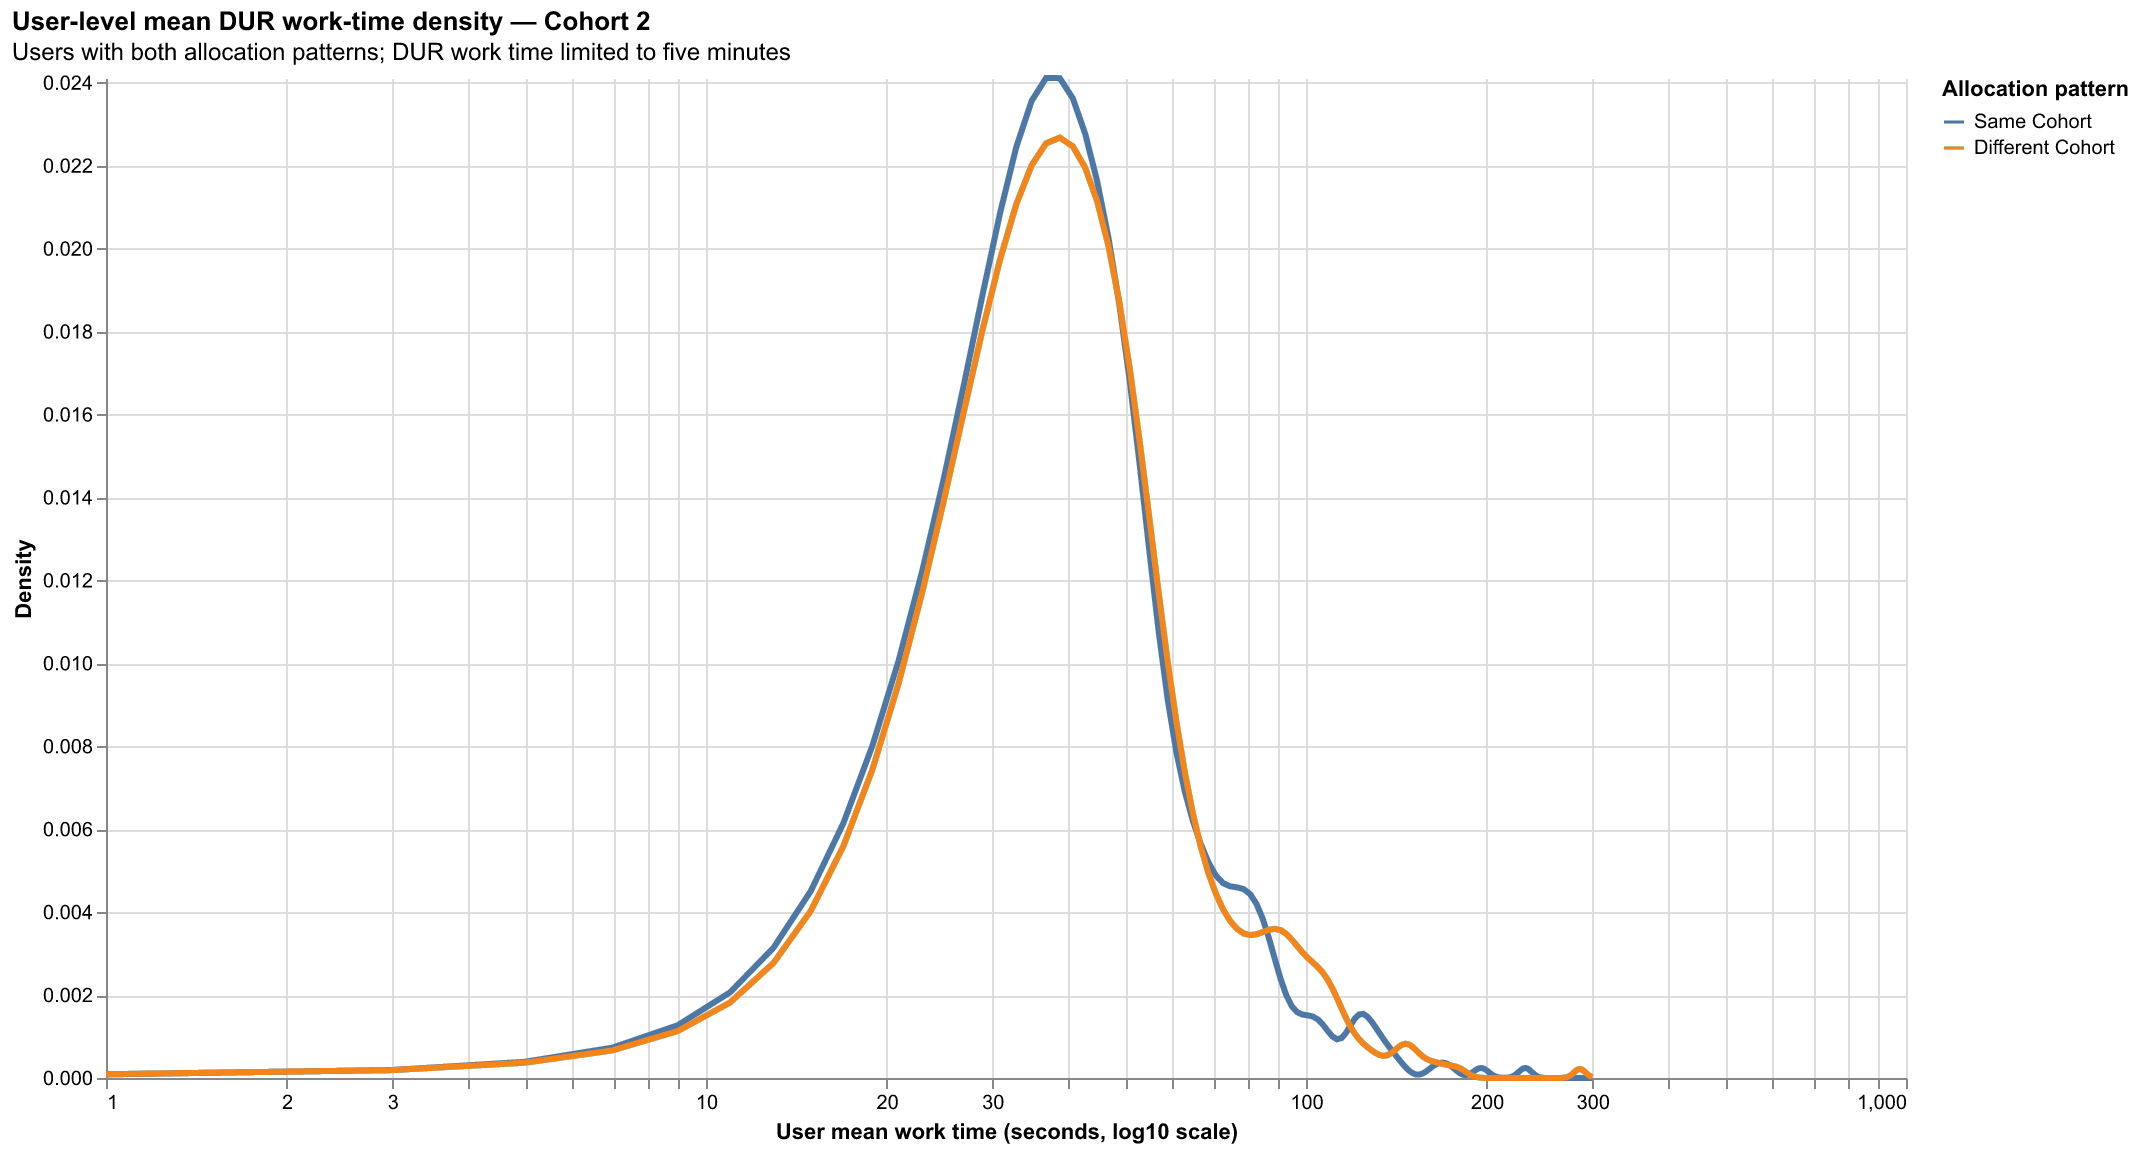
\includegraphics[width=\dimexpr\linewidth-2\fboxsep-2\fboxrule\relax,keepaspectratio,alt={User-level work-time density for Cohort 2}]{outputs/charts/stats-comparison-user/stats-comparison-user-cohort-2.png}}
\captionof{figure}{User-level work-time density, Cohort 2.}\label{fig:cohort-user-one-sided-2}
\end{minipage}

\vspace{0.7em}
\begin{minipage}[t]{0.49\linewidth}
\vspace{0pt}\centering
\fbox{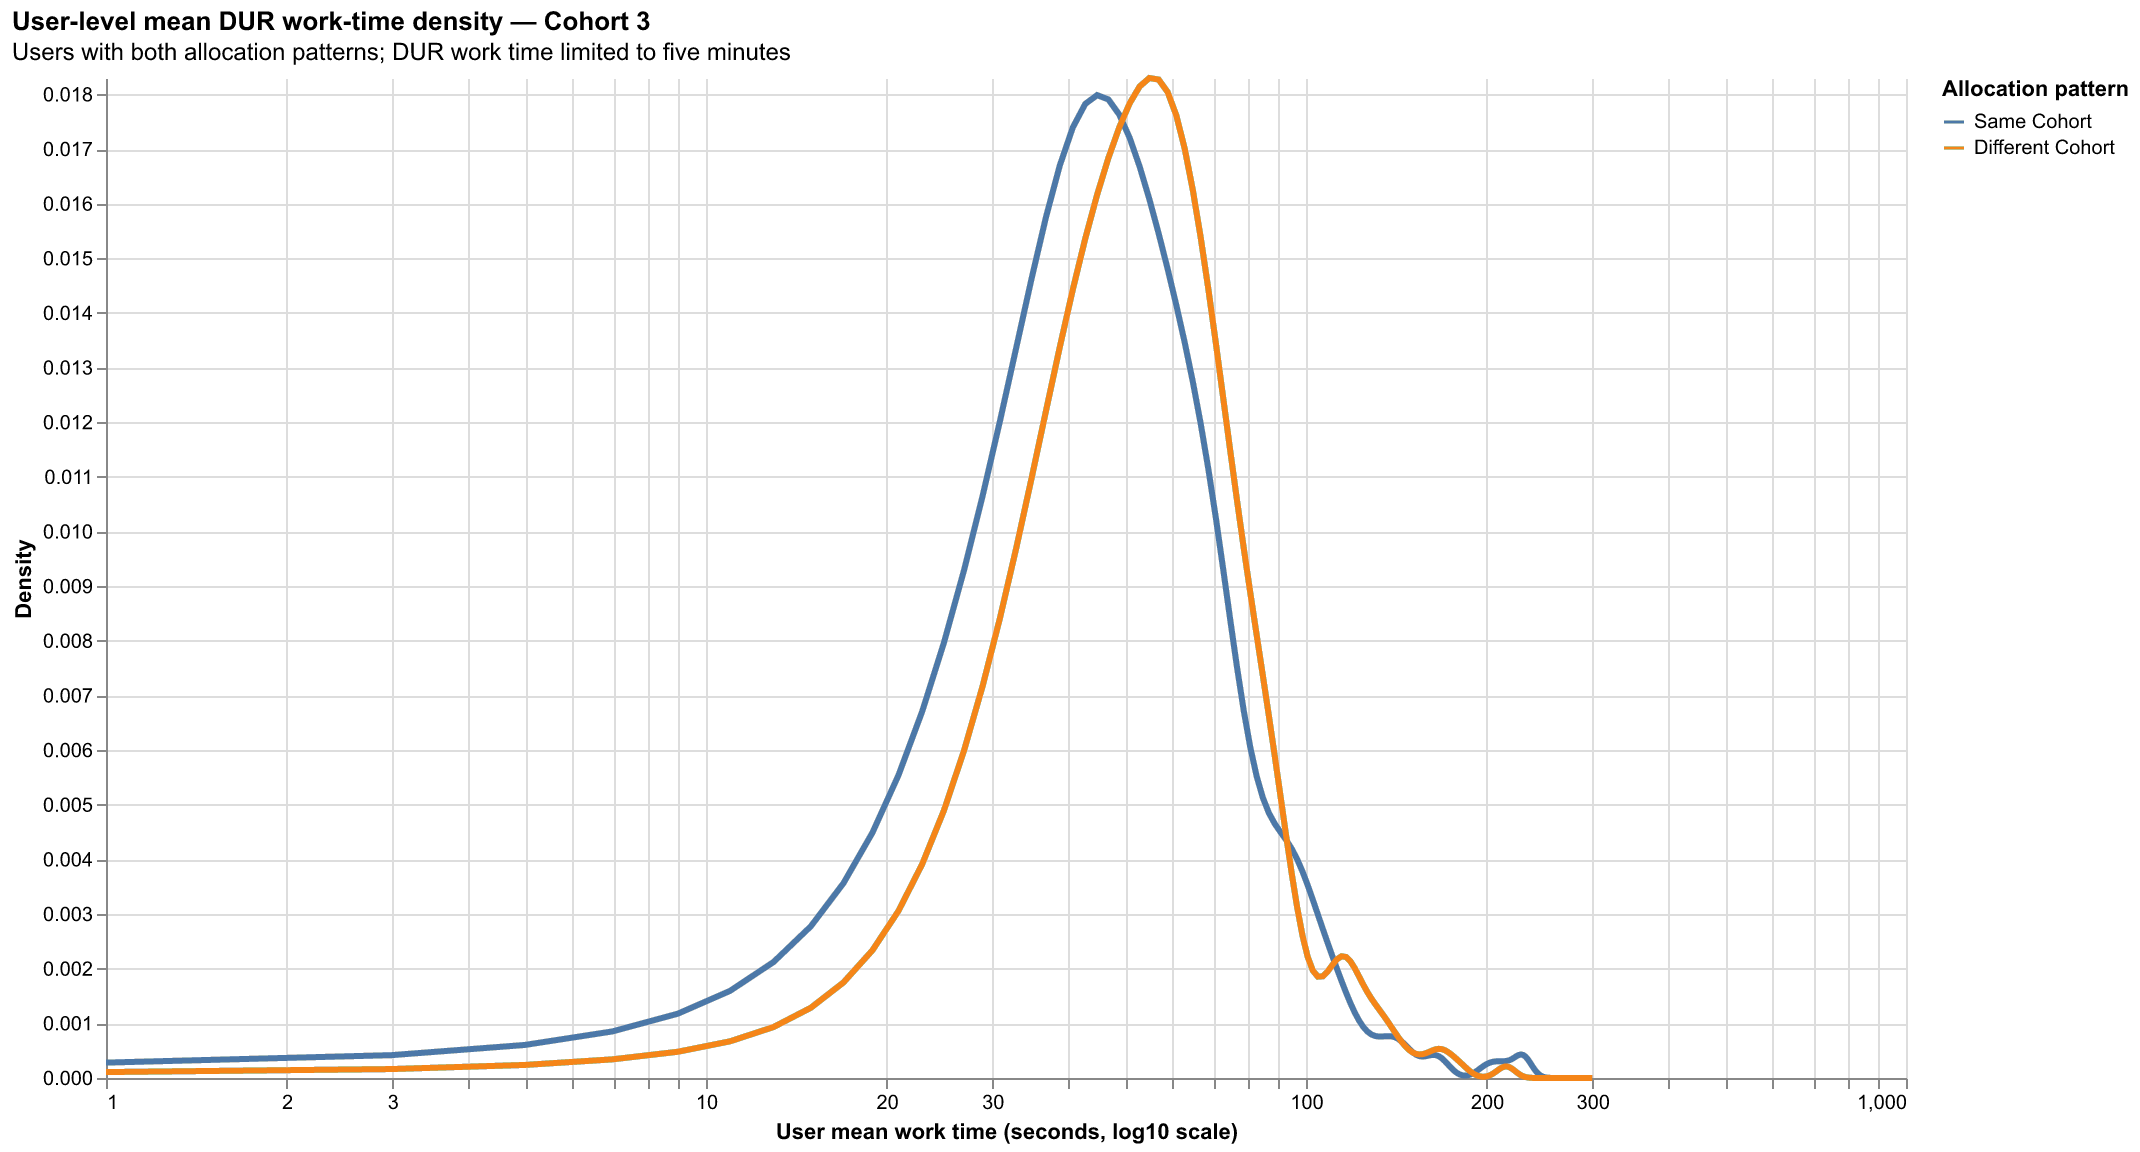
\includegraphics[width=\dimexpr\linewidth-2\fboxsep-2\fboxrule\relax,keepaspectratio,alt={User-level work-time density for Cohort 3}]{outputs/charts/stats-comparison-user/stats-comparison-user-cohort-3.png}}
\captionof{figure}{User-level work-time density, Cohort 3.}\label{fig:cohort-user-one-sided-3}
\end{minipage}\hfill
\begin{minipage}[t]{0.49\linewidth}
\vspace{0pt}\centering
\fbox{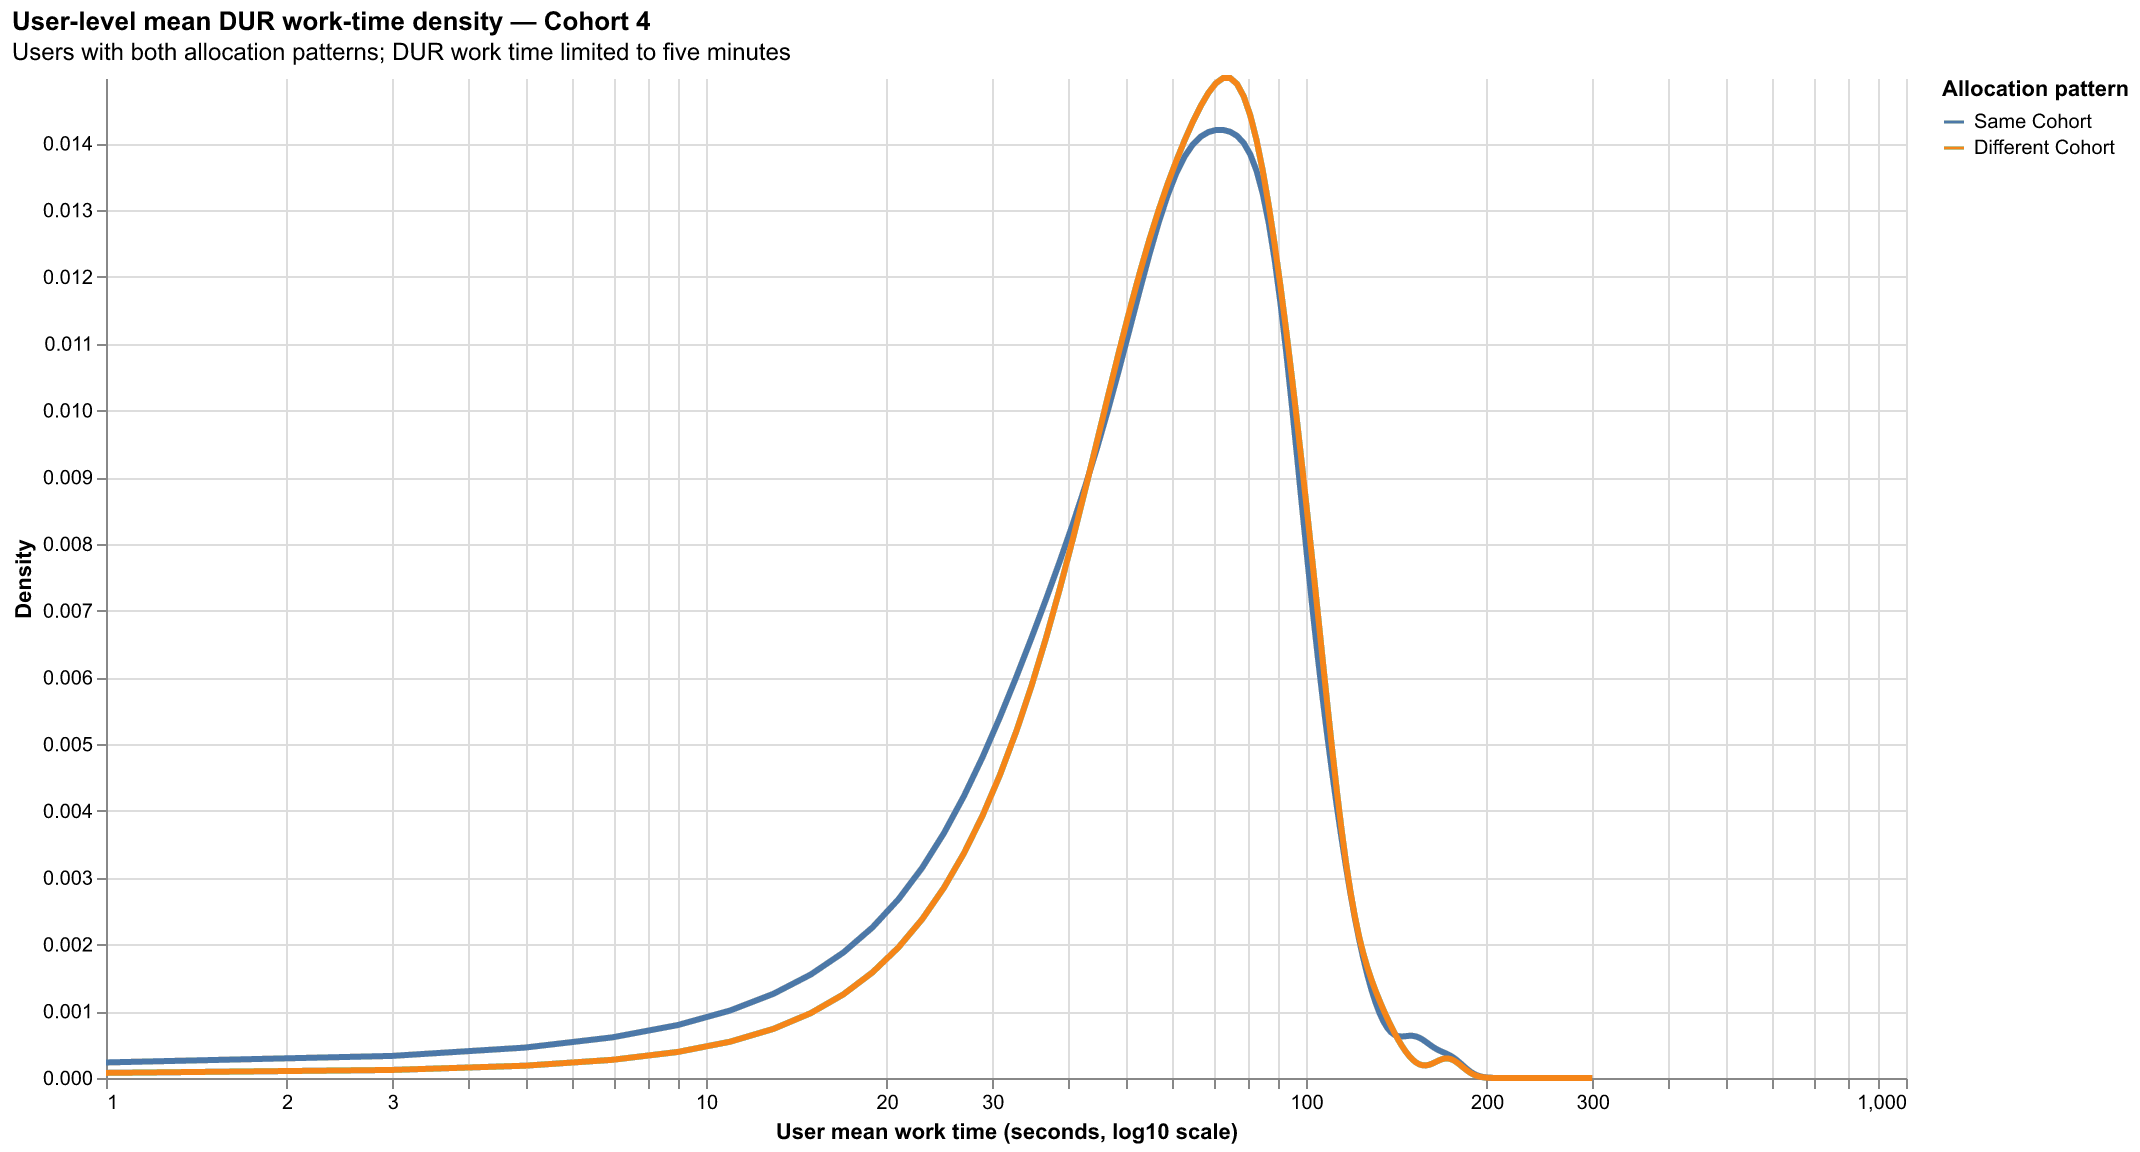
\includegraphics[width=\dimexpr\linewidth-2\fboxsep-2\fboxrule\relax,keepaspectratio,alt={User-level work-time density for Cohort 4}]{outputs/charts/stats-comparison-user/stats-comparison-user-cohort-4.png}}
\captionof{figure}{User-level work-time density, Cohort 4.}\label{fig:cohort-user-one-sided-4}
\end{minipage}
\end{minipage}
\end{center}

\subsubsection{Cohort results}
Table~\ref{tab:cohort-user-pattern-summary} reports the distribution of
user-level mean work times. The same matched users contribute to both rows
for each cohort.

\begin{center}
\begin{minipage}{\linewidth}
\centering\fontsize{8}{10}\selectfont
\begin{tabular}{@{}llrrlrrrr@{}}
\toprule
Cohort & Allocation pattern & Users & \shortstack{Mean user\\mean (min)} & \shortstack{95\% CI for mean\\(min)} & SD & Median & P25 & P75 \\
\midrule
1 & Same Cohort      & 289 & 0.6681 & $[0.6193,0.7170]$ & 0.4217 & 0.5410 & 0.4329 & 0.7469 \\
1 & Different Cohort & 289 & 0.7308 & $[0.6703,0.7912]$ & 0.5220 & 0.5909 & 0.4648 & 0.7776 \\
2 & Same Cohort      & 286 & 0.8402 & $[0.7831,0.8974]$ & 0.4910 & 0.7114 & 0.5552 & 0.9312 \\
2 & Different Cohort & 286 & 0.8767 & $[0.8155,0.9380]$ & 0.5259 & 0.7445 & 0.5660 & 0.9848 \\
3 & Same Cohort      & 250 & 1.0091 & $[0.9399,1.0783]$ & 0.5552 & 0.8809 & 0.6676 & 1.1693 \\
3 & Different Cohort & 250 & 1.0650 & $[1.0054,1.1247]$ & 0.4785 & 0.9695 & 0.7510 & 1.2296 \\
4 & Same Cohort      & 139 & 1.2037 & $[1.1285,1.2790]$ & 0.4488 & 1.1814 & 0.9098 & 1.4688 \\
4 & Different Cohort & 139 & 1.2202 & $[1.1504,1.2899]$ & 0.4161 & 1.2020 & 0.9106 & 1.4989 \\
\bottomrule
\end{tabular}
\captionof{table}{User-level mean DUR work time by cohort and allocation pattern.}\label{tab:cohort-user-pattern-summary}
\end{minipage}
\end{center}

The paired comparison uses the within-user difference
$\text{Same Cohort}-\text{Different Cohort}$. Table~\ref{tab:cohort-user-paired-test}
gives the one-sided test results. At the 0.05 level, the null hypothesis is
rejected for Cohorts 1--3 but not for Cohort 4.

\begin{center}
\begin{minipage}{\linewidth}
\centering\fontsize{8}{10}\selectfont
\begin{tabular}{@{}rrrllrrl@{}}
\toprule
Cohort & Users & \shortstack{Mean difference\\(min)} & \shortstack{95\% two-sided CI\\(min)} & \shortstack{95\% one-sided\\upper bound} & $t$ & df & One-sided $p$ \\
\midrule
1 & 289 & $-0.0626$ & $[-0.0972,-0.0281]$ & $(-\infty,-0.0337]$ & $-3.5706$ & 288 & 0.000208592 \\
2 & 286 & $-0.0365$ & $[-0.0703,-0.0028]$ & $(-\infty,-0.0082]$ & $-2.1302$ & 285 & 0.0170078 \\
3 & 250 & $-0.0559$ & $[-0.1043,-0.0075]$ & $(-\infty,-0.0154]$ & $-2.2766$ & 249 & 0.0118295 \\
4 & 139 & $-0.0164$ & $[-0.0557,0.0229]$  & $(-\infty,0.0165]$  & $-0.8272$ & 138 & 0.204771 \\
\bottomrule
\end{tabular}
\captionof{table}{One-sided paired tests of Same Cohort minus Different Cohort mean work time.}\label{tab:cohort-user-paired-test}
\end{minipage}
\end{center}

\subsubsection{Data}
The data is obtained using the following query.

\begingroup\fontsize{8}{9}\selectfont
\begin{verbatim}
WITH ordered AS (
  SELECT
    TASK_ID, USER_ID, ITEM_COHORT, STARTED_AT,
    TRANSITION_STARTED_AT::DATE AS dt,
    LAG(ITEM_COHORT) OVER (
      PARTITION BY USER_ID, TRANSITION_STARTED_AT::DATE
      ORDER BY STARTED_AT
    ) AS prev_cohort,
    DWELL_IN_PROGRESS_TO_CLOSED_MINUTES AS work_min
  FROM EDLDB.PET_HEALTH_ANALYTICS_SANDBOX.FCT__TASKS_LIFECYCLE
  WHERE TRANSITION_STARTED_AT >= '2026-08-01'
    AND TASK_TYPE = 'DUR' AND FINAL_STATUS = 'CLOSED'
    AND USER_ID IS NOT NULL AND STARTED_AT IS NOT NULL
    AND DWELL_IN_PROGRESS_TO_CLOSED_MINUTES BETWEEN 0.01 AND 5
    AND ITEM_COHORT != 'Unknown'
)
SELECT
  TASK_ID AS task_id, USER_ID AS user_id, dt,
  CASE
    WHEN ITEM_COHORT = prev_cohort THEN 'Same Cohort'
    ELSE 'Different Cohort'
  END AS allocation_pattern,
  ITEM_COHORT AS cohort, work_min
FROM ordered
WHERE prev_cohort IS NOT NULL
ORDER BY allocation_pattern, work_min
\end{verbatim}
\endgroup

\subsection{Modeling DUR Processing Time}\label{modeling-dur-processing-time}

A model was built to predict DUR durations for the following reasons:

\begin{itemize}
\tightlist
\item
  The analysis
  \href{https://chewyinc.atlassian.net/wiki/x/hYRyRQE}{Would Grouping
  Similar Work Make Pharmacists Faster? What the data says} concludes
  that the previous task has no effect. We would like to know whether
  the result changes after controlling for factors other than MC3,
  cohort, or part number. We also want to determine whether another
  definition of similarity is more appropriate and quantify the
  uncertainty in the estimate.
\end{itemize}

Consider two task sequences from the same user:

Both sequences have MC3 \texttt{Parasiticide} and approval channel
\texttt{PH}. All start times have UTC offset \texttt{+0000} and
\texttt{.000} milliseconds; blank updated fields mean no fields were
updated.

Sequence A: pet \texttt{Dog}, initiation channel \texttt{AUTOSHIP}.

{\def\LTcaptype{none} % do not increment counter
\begin{longtable}[]{@{}rrrll@{}}
\toprule\noalign{}
Order & Part number & Duration (s) & Start time (UTC) & Updated
fields \\
\midrule\noalign{}
\endhead
\bottomrule\noalign{}
\endlastfoot
1 & 146066 & 40 & 2026-04-30 06:42:54 & \\
2 & 152702 & 27 & 2026-04-30 06:43:36 & directions \\
3 & 146391 & 40 & 2026-04-30 06:44:06 & \\
4 & 151583 & 7 & 2026-04-30 06:44:48 & \\
5 & 146138 & 7 & 2026-04-30 06:44:56 & \\
6 & 146142 & 43 & 2026-04-30 06:45:05 & directions \\
7 & 146142 & 35 & 2026-04-30 06:45:49 & directions \\
8 & 146064 & 39 & 2026-04-30 06:46:26 & directions \\
9 & 146167 & 12 & 2026-04-30 06:47:07 & \\
10 & 146322 & 9 & 2026-04-30 06:47:21 & directions \\
11 & 146167 & 97 & 2026-04-30 06:47:32 & directions \\
12 & 146050 & 6 & 2026-04-30 06:49:11 & \\
13 & 146387 & 54 & 2026-04-30 06:49:19 & \\
\end{longtable}
}

Sequence B: pet \texttt{Cat}, initiation channel \texttt{OMS}.

{\def\LTcaptype{none} % do not increment counter
\begin{longtable}[]{@{}rrrll@{}}
\toprule\noalign{}
Order & Part number & Duration (s) & Start time (UTC) & Updated
fields \\
\midrule\noalign{}
\endhead
\bottomrule\noalign{}
\endlastfoot
1 & 158995 & 11 & 2026-07-15 02:17:23 & \\
2 & 158995 & 35 & 2026-07-15 02:17:36 & \\
3 & 158995 & 3 & 2026-07-15 02:18:13 & \\
4 & 158995 & 13 & 2026-07-15 02:18:17 & \\
5 & 158995 & 13 & 2026-07-15 02:18:31 & \\
6 & 158995 & 6 & 2026-07-15 02:18:46 & \\
7 & 158995 & 16 & 2026-07-15 02:18:53 & \\
8 & 158995 & 13 & 2026-07-15 02:19:11 & \\
9 & 158995 & 6 & 2026-07-15 02:19:25 & \\
10 & 158995 & 50 & 2026-07-15 02:19:32 & \\
11 & 158998 & 11 & 2026-07-15 02:20:23 & \\
12 & 158998 & 29 & 2026-07-15 02:20:36 & \\
\end{longtable}
}

The model predicts a statistically significant effect when the preceding
task is "similar" for a user. However, substantial unexplained variation
remains.

The predicted effect at several baseline DUR durations is:

\begingroup\setlength{\tabcolsep}{5pt}

{\def\LTcaptype{none} % do not increment counter
\begin{longtable}[]{@{}rrrrrr@{}}
\toprule\noalign{}
Without same preceding & With same preceding & -1 residual SD & +1
residual SD & Difference & Change (\%) \\
\midrule\noalign{}
\endhead
\bottomrule\noalign{}
\endlastfoot
15.00 s & 14.16 s & 6.84 s & 30.70 s & -0.84 s & -5.58\% \\
50.00 s & 46.93 s & 21.09 s & 110.44 s & -3.07 s & -6.14\% \\
150.00 s & 139.96 s & 58.53 s & 357.84 s & -10.04 s & -6.69\% \\
\end{longtable}
}

\endgroup

The model predicts that users and products differ in processing speed,
while day of the week has no statistically significant effect.

The model also predicts longer DUR times when prescription data are
altered.

How reliable are our estimates for hypothetical sequencing scenarios?

\subsubsection{EDA on Factors Affecting
DUR}\label{eda-on-factors-affecting-dur}

See \hyperref[factors-affecting-successful-durs]{Factors Affecting DUR}
in the Appendix.

We assume that the following groups of factors affect DUR duration:

\begin{enumerate}
\def\labelenumi{\arabic{enumi}.}
\tightlist
\item
  The user

  \begin{itemize}
  \tightlist
  \item
    Are some users inherently slower? Are they consistently slower or
    faster across cohorts?
  \end{itemize}
\item
  The prescription

  \begin{itemize}
  \tightlist
  \item
    Medication
  \item
    Content (typos, missing information)
  \item
    Pet

    \begin{itemize}
    \tightlist
    \item
      Pet health history
    \end{itemize}
  \end{itemize}
\item
  Business process
\item
  Outside disturbances, such as inbound calls
\item
  The user\textquotesingle s task history

  \begin{itemize}
  \tightlist
  \item
    Did they perform similar tasks previously?
  \end{itemize}
\item
  Environment
\item
  Software platform
\end{enumerate}

A more detailed breakdown can be found
\href{../../charts/DUR_detailed.png}{here}.

For details, see \hyperref[model-details]{Model Details} in the
Appendix.


\paragraph{Model Details}\label{model-details}

\subparagraph{Final MC3/COH/PETTYPE mixed-effects
model}\label{final-mc3cohpettype-mixed-effects-model}

The model is built to understand the factors affecting approved DUR task
durations. It uses MC3, cohort, and pet type to define groups of similar
DUR tasks.

The model controls for weekday, approval channel, prescription source,
parent part number, user (for example, pharmacist or pharmacy
technician), and changes to prescription data, such as updated
directions.

There are two treatments based on whether the current task is adjacent
to another task in the same MC3, cohort, and pet type equivalence class
for a given user. Adjacent tasks must be no more than one hour apart.
Failed DURs and DUR tasks that overlap in time with other DUR tasks are
excluded; these cases occur for certain orders. If a preceding task
belongs to the same equivalence class, the \texttt{SAME\_PRECEDING}
treatment is true. If the following task belongs to the same equivalence
class, the \texttt{SAME\_FOLLOWING} treatment is true.
\texttt{SAME\_FOLLOWING} is expected to have a coefficient near zero. It
exists to check whether the model captures confounding factors
adequately.

The model estimates each user\textquotesingle s deviation from mean
performance. It does the same for each parent part number and each
calendar date.

The model predicts that, for a given user, a task preceded by a task in
the same cell has a shorter DUR duration. After controlling for MC3,
cohort, pet type, and parent part number, the model finds no
statistically significant association with \texttt{SAME\_FOLLOWING}.

The weekday fixed effects are not statistically significant, whereas
some approval-channel and prescription-source effects are.
Customer-originated prescriptions take longer.

\subparagraph{Purpose and analysis
sample}\label{purpose-and-analysis-sample}

This is the final model. It estimates how same-cell sequence position
relates to DUR duration while controlling for correction status,
weekday, approval channel, prescription source, and MC3/COH/PETTYPE
cell. It includes crossed random intercepts for user, process date, and
parent part number.

The source is
\texttt{EDLDB\_DEV.PET\_HEALTH\_ANALYTICS\_SANDBOX.MY\_RXP\_VALID\_DUR\_TASKS}.
Eligible rows have non-null user, task, process-start time,
\texttt{MC3\_COH\_PETTYPE\_SEQN}, and
\texttt{MC3\_COH\_PETTYPE\_BATCH\_LEN}; sequence and batch length are at
least one, and sequence does not exceed batch length. Duration is
\texttt{IMPUTED\_DWELL\_IN\_PROGRESS\_TO\_CLOSED\_SECONDS}.

Let \(Y_i\) be the positive imputed duration in seconds for task \(i\).
One global cutoff is calculated over all otherwise eligible tasks with
Snowflake\textquotesingle s \texttt{APPROX\_PERCENTILE(Y,\ 0.95)}
function call:

\[
q_{0.95}=Q_{0.95}(Y).
\]

The fitted sample keeps tasks satisfying \(0<Y_i<q_{0.95}\); the upper
bound is strict. MC3, COH, PETTYPE, parent part number, approval
channel, and prescription source blanks are represented by
\texttt{\textless{}Missing\textgreater{}}.

\subparagraph{Derived indicators}\label{derived-indicators}

For sequence number \(S_i\), batch length \(L_i\), and correction count
\(N_i\), the three binary fixed effects are

\[
P_i=\mathbf{1}(L_i>1\ \land\ S_i>1),
\qquad
F_i=\mathbf{1}(L_i>1\ \land\ S_i<L_i),
\qquad
C_i=\mathbf{1}(N_i>0).
\]

Thus \(P_i\) is \texttt{SAME\_PRECEDING}, \(F_i\) is
\texttt{SAME\_FOLLOWING}, and \(C_i\) is \texttt{HAS\_CORRECTION}.

\subparagraph{Outcome transformation}\label{outcome-transformation}

The retained durations receive one global Box-Cox transformation:

\[
Z_i=g_\lambda(Y_i)=
\begin{cases}
\dfrac{Y_i^\lambda-1}{\lambda}, & \lambda\ne0,\\
\log(Y_i), & \lambda=0.
\end{cases}
\]

The maximum-likelihood transformation estimate is
\(\widehat{\lambda}=-0.08159843\). All coefficients, random effects,
standard deviations, residuals, RMSE, and diagnostics are therefore on
the Box-Cox scale.

\subparagraph{Complete model formula}\label{complete-model-formula}

Index task, fixed-effect cell, user, date, and parent part by
\(i, c, u, d, p\). The model is

\[
\begin{aligned}
Z_i={}&\gamma_{c(i)}+\beta_P P_i+\beta_F F_i+\beta_C C_i\\
&+\sum_{w\ne\mathrm{Sun}}\delta_w\mathbf{1}(W_i=w)\\
&+\sum_{a\ne a_0}\theta_a\mathbf{1}(A_i=a)
+\sum_{s\ne s_0}\phi_s\mathbf{1}(R_i=s)\\
&+b_{u(i)}+h_{d(i)}+r_{p(i)}+\epsilon_i.
\end{aligned}
\]

Here \(\gamma_{c(i)}\) is a fixed effect shared by all tasks in the same
MC3 + COH + PETTYPE cell. The model uses a full set of cell effects and
no separate overall intercept. Sunday is the weekday reference. The
data-dependent categorical references are:

\begin{itemize}
\tightlist
\item
  approval channel \(a_0\): \texttt{PH}
\item
  prescription source \(s_0\): \texttt{PRACTICE\_HUB}
\end{itemize}

Each reference is the most frequent retained level; lexicographic order
breaks a frequency tie. The crossed random terms and level-1 error are
mutually independent and satisfy

\[
b_u\sim N(0,\sigma_u^2),\qquad
h_d\sim N(0,\sigma_d^2),\qquad
r_p\sim N(0,\sigma_p^2),\qquad
\epsilon_i\sim N(0,\sigma_e^2).
\]

The fixed effects and variance components are estimated jointly by REML.
The conditional fitted value and residual are

\[
\widehat{Z}_i=\widehat{\gamma}_{c(i)}+x_i^T\widehat{\beta}
+\widehat{b}_{u(i)}+\widehat{h}_{d(i)}+\widehat{r}_{p(i)},
\qquad e_i=Z_i-\widehat{Z}_i.
\]

\subparagraph{Inference and fit
statistics}\label{inference-and-fit-statistics}

For fixed effect \(k\), the report uses

\[
z_k=\frac{\widehat{\beta}_k}{\mathrm{SE}(\widehat{\beta}_k)},\qquad
p_k=2\Phi(-\lvert z_k\rvert),\qquad
\mathrm{CI}_{95}=\widehat{\beta}_k\pm1.96\,\mathrm{SE}(\widehat{\beta}_k).
\]

The fixed-effect table labels an estimate \texttt{Significant\ =\ Yes}
when its 95\% confidence interval excludes zero; intervals that cross or
touch zero are marked \texttt{No}.

Random-effect SD intervals use an observed-information Wald
approximation on the log-SD scale. The residual-SD interval uses the
chi-square distribution. The reported conditional metrics include all
fixed and random effects:

\[
R_c^2=1-\frac{\sum_i e_i^2}{\sum_i(Z_i-\bar Z)^2},\qquad
RMSE_c=\sqrt{\frac1n\sum_i e_i^2}.
\]

\Needspace{8\baselineskip}

\subparagraph{Sample and fit}\label{sample-and-fit}

{\def\LTcaptype{none} % do not increment counter
\begin{longtable}[]{@{}lr@{}}
\toprule\noalign{}
Quantity & Value \\
\midrule\noalign{}
\endhead
\bottomrule\noalign{}
\endlastfoot
Tasks & 3,433,218 \\
MC3/COH/PETTYPE cells & 265 \\
Users & 340 \\
Dates & 182 \\
Parent part numbers & 885 \\
Approval-channel levels & 9 \\
Prescription-source levels & 11 \\
Global approximate P95 cutoff (seconds) & 156.598673 \\
Box-Cox lambda & -0.08159843 \\
Conditional R-squared & 0.308784 \\
Conditional RMSE (Box-Cox scale) & 0.603674 \\
REML negative log-likelihood & 3142827.127402 \\
Converged & True \\
\end{longtable}
}

\subparagraph{Fixed effects}\label{fixed-effects}

In the term column, \texttt{AC} denotes approval-channel effects
relative to \texttt{PH}; \texttt{PS} denotes prescription-source effects
relative to \texttt{PRACTICE\_HUB}.

\begingroup\setlength{\tabcolsep}{4pt}

{\def\LTcaptype{none} % do not increment counter
\begin{longtable}[]{@{}lrrrrrc@{}}
\toprule\noalign{}
Term & Estimate & SE & z & p-value & 95\% CI & Significant \\
\midrule\noalign{}
\endhead
\bottomrule\noalign{}
\endlastfoot
SAME\_PRECEDING & -0.046157 & 0.000835 & -55.2813 & \textless1e-300 &
{[}-0.047793, -0.044520{]} & Yes \\
SAME\_FOLLOWING & 0.001024 & 0.000835 & 1.2259 & 0.220231 &
{[}-0.000613, 0.002661{]} & No \\
HAS\_CORRECTION & 0.271146 & 0.000788 & 344.0672 & \textless1e-300 &
{[}0.269601, 0.272690{]} & Yes \\
WEEKDAY\_MON & 0.006416 & 0.019649 & 0.3265 & 0.74404 & {[}-0.032096,
0.044927{]} & No \\
WEEKDAY\_TUE & 0.014299 & 0.019646 & 0.7278 & 0.466718 & {[}-0.024206,
0.052803{]} & No \\
WEEKDAY\_WED & 0.010462 & 0.019650 & 0.5324 & 0.59444 & {[}-0.028051,
0.048975{]} & No \\
WEEKDAY\_THU & 0.008138 & 0.019652 & 0.4141 & 0.678785 & {[}-0.030379,
0.046655{]} & No \\
WEEKDAY\_FRI & 0.006015 & 0.019651 & 0.3061 & 0.75952 & {[}-0.032499,
0.044530{]} & No \\
WEEKDAY\_SAT & 0.002131 & 0.019666 & 0.1084 & 0.913702 & {[}-0.036413,
0.040675{]} & No \\
AC: CLINIC\_EMAIL & 0.235910 & 0.045211 & 5.2180 & 1.80853e-07 &
{[}0.147299, 0.324522{]} & Yes \\
AC: CUSTOMER\_MAIL & 0.472534 & 0.013061 & 36.1785 & 1.32431e-286 &
{[}0.446934, 0.498133{]} & Yes \\
AC: DIGITAL & 0.146802 & 0.040724 & 3.6048 & 0.000312369 & {[}0.066985,
0.226619{]} & Yes \\
AC: FAX & 0.208015 & 0.011227 & 18.5276 & 1.23668e-76 & {[}0.186010,
0.230020{]} & Yes \\
AC: PARTNER & -0.034275 & 0.007967 & -4.3018 & 1.69381e-05 &
{[}-0.049891, -0.018659{]} & Yes \\
AC: RHAPSODY & 0.075320 & 0.052573 & 1.4327 & 0.15195 & {[}-0.027721,
0.178362{]} & No \\
AC: VERBAL & -0.017687 & 0.010665 & -1.6585 & 0.097222 & {[}-0.038589,
0.003215{]} & No \\
AC: VET & 0.003570 & 0.105720 & 0.0338 & 0.973059 & {[}-0.203638,
0.210779{]} & No \\
PS: CLINIC\_EMAIL & -0.003227 & 0.011181 & -0.2886 & 0.772878 &
{[}-0.025141, 0.018687{]} & No \\
PS: CS\_FIRST\_CONTACT & -0.086051 & 0.203897 & -0.4220 & 0.673003 &
{[}-0.485682, 0.313580{]} & No \\
PS: CUSTOMER\_MAIL & 0.044423 & 0.012813 & 3.4672 & 0.000525987 &
{[}0.019311, 0.069536{]} & Yes \\
PS: CVC & 0.023167 & 0.052511 & 0.4412 & 0.659085 & {[}-0.079753,
0.126087{]} & No \\
PS: DIGITAL & 0.020414 & 0.040106 & 0.5090 & 0.610753 & {[}-0.058192,
0.099020{]} & No \\
PS: FAX & -0.004739 & 0.011224 & -0.4222 & 0.67286 & {[}-0.026738,
0.017260{]} & No \\
PS: PARTNER\_API & 0.018961 & 0.007944 & 2.3869 & 0.0169906 &
{[}0.003392, 0.034530{]} & Yes \\
PS: RHAPSODY & -0.029700 & 0.062733 & -0.4734 & 0.6359 & {[}-0.152655,
0.093254{]} & No \\
PS: TELEMEDICINE & 0.185396 & 0.052942 & 3.5018 & 0.000462051 &
{[}0.081631, 0.289161{]} & Yes \\
PS: VERBAL & -0.002803 & 0.011736 & -0.2388 & 0.81126 & {[}-0.025805,
0.020200{]} & No \\
\end{longtable}
}

\endgroup

\Needspace{8\baselineskip}

\subparagraph{Variance components}\label{variance-components}

{\def\LTcaptype{none} % do not increment counter
\begin{longtable}[]{@{}lrr@{}}
\toprule\noalign{}
Component & SD & Approximate 95\% CI \\
\midrule\noalign{}
\endhead
\bottomrule\noalign{}
\endlastfoot
User random intercept & 0.422318 & {[}0.390500, 0.456728{]} \\
Date random intercept & 0.070610 & {[}0.063513, 0.078500{]} \\
Parent-part random intercept & 0.114187 & {[}0.107719, 0.121045{]} \\
Residual & 0.603803 & {[}0.603351, 0.604255{]} \\
\end{longtable}
}

\subparagraph{Diagnostics}\label{diagnostics}

\pandocbounded{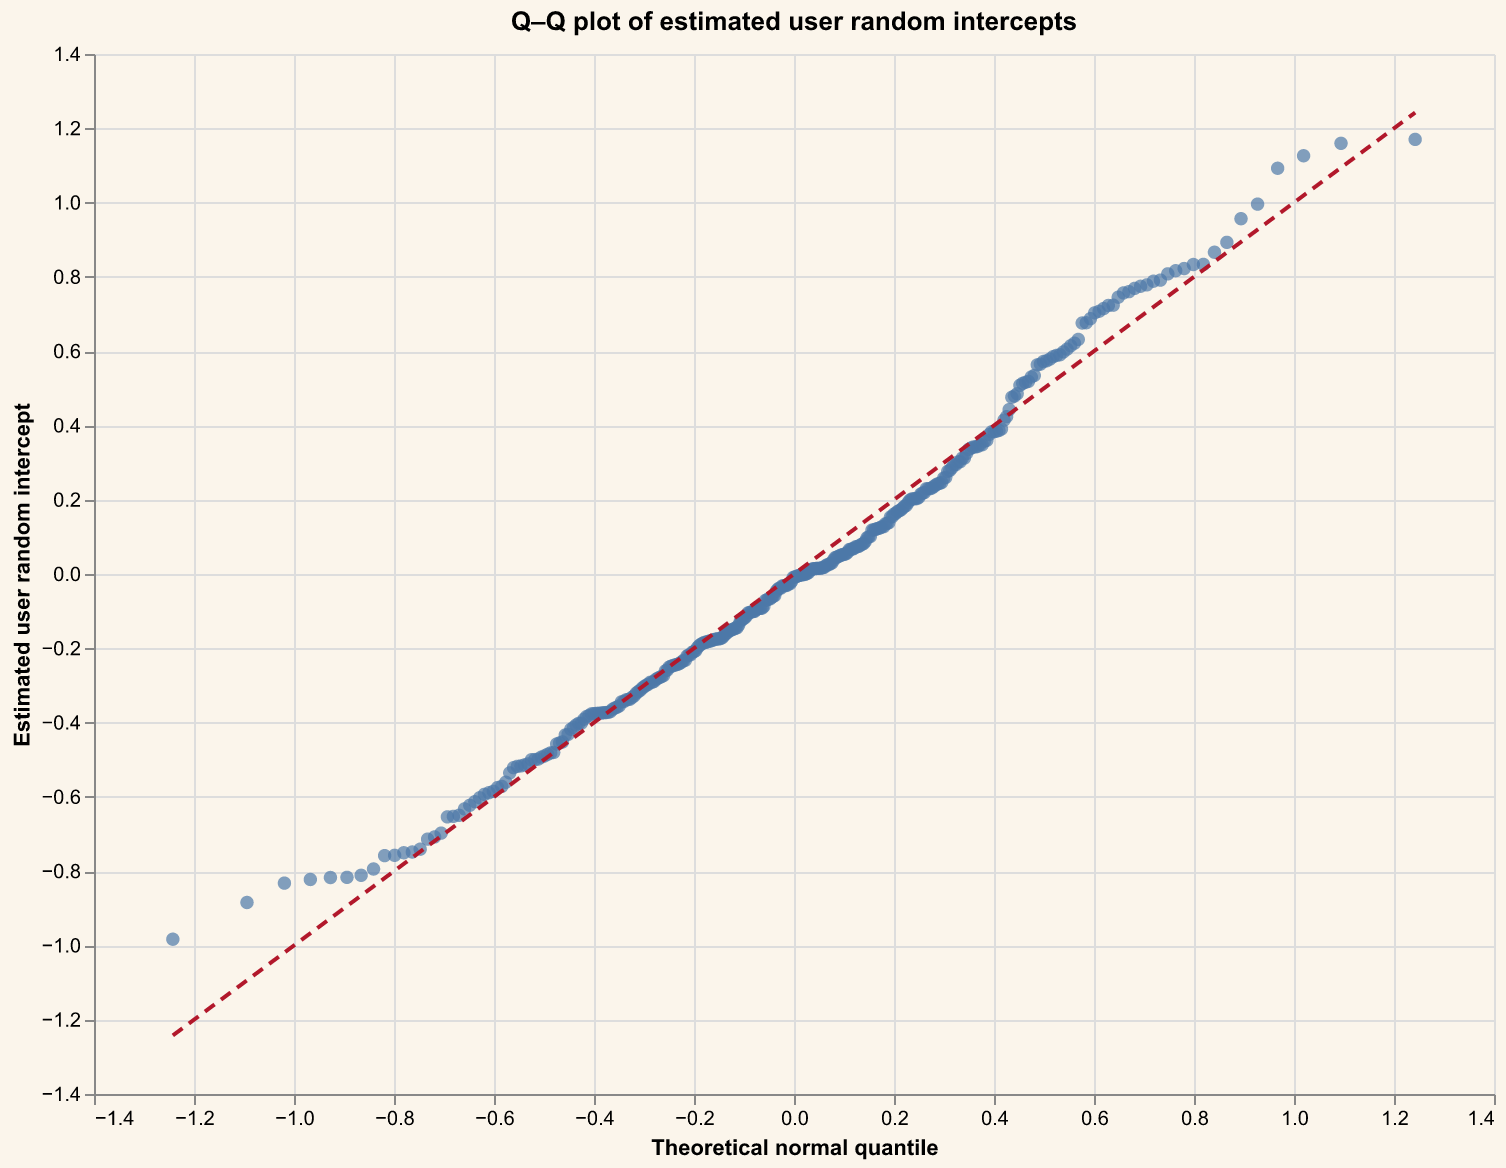
\includegraphics[keepaspectratio,alt={User Q--Q plot}]{outputs/charts/mc3-coh-pettype-final-model/user_random_intercepts_qq.png}}

\pandocbounded{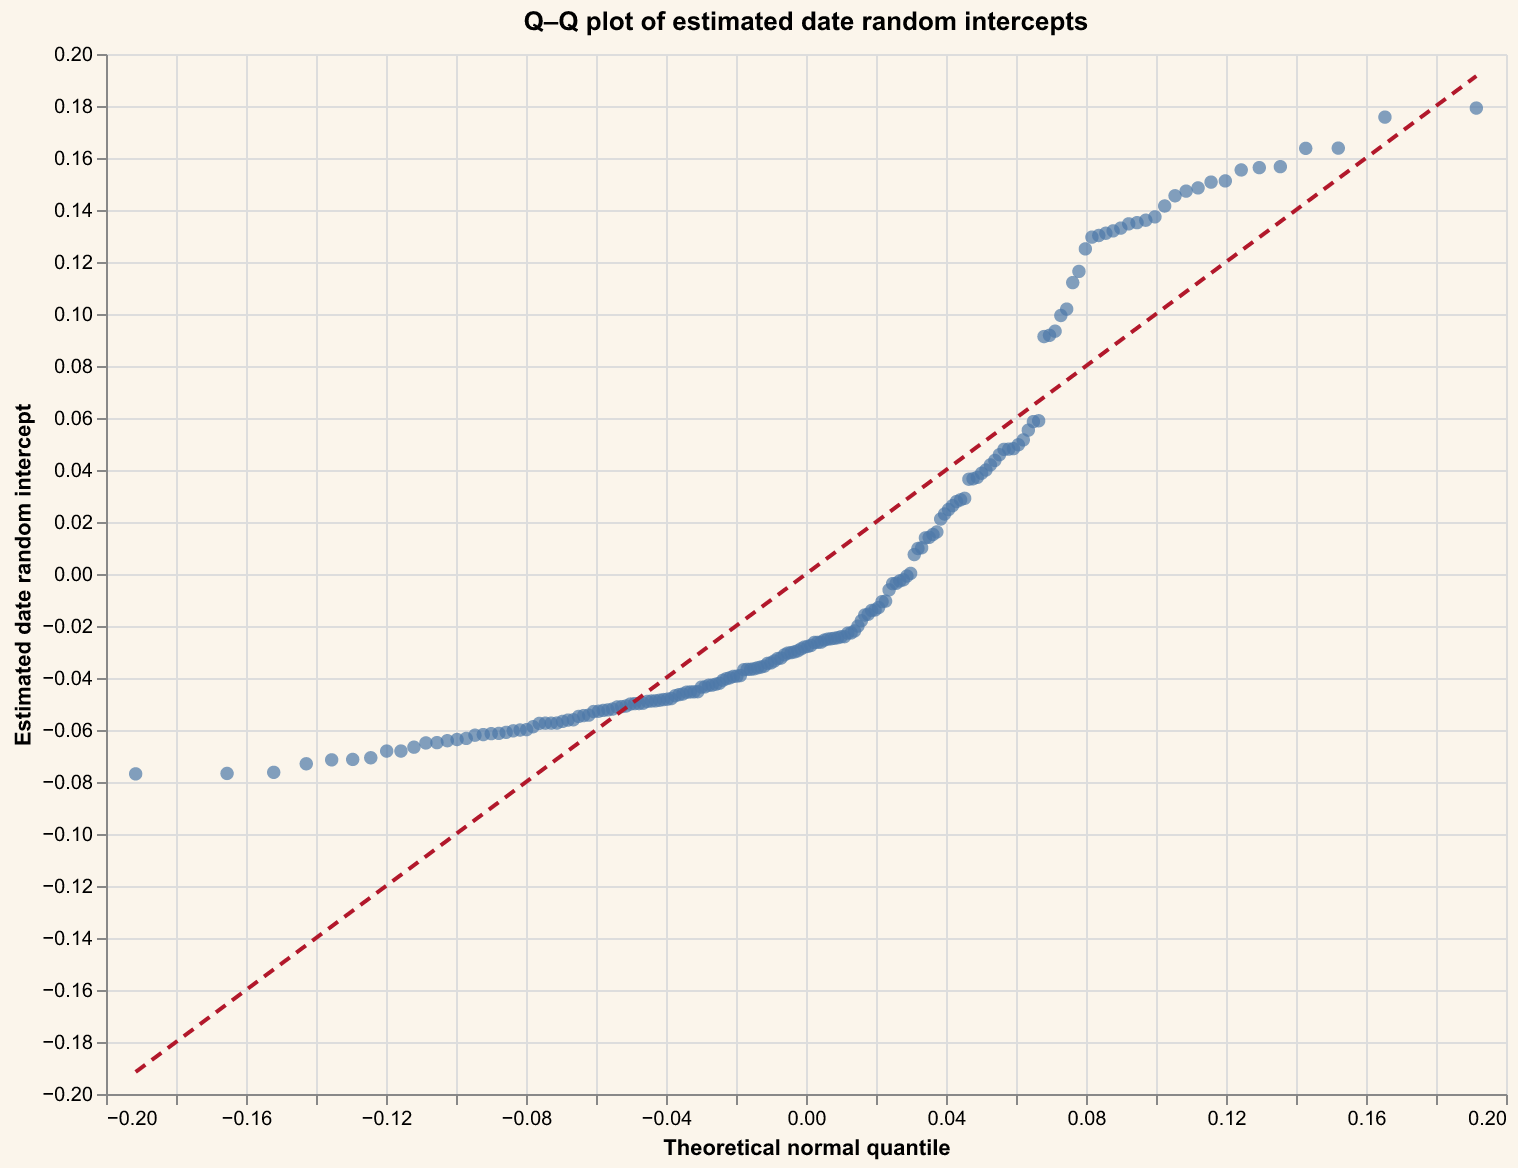
\includegraphics[keepaspectratio,alt={Date Q--Q plot}]{outputs/charts/mc3-coh-pettype-final-model/date_random_intercepts_qq.png}}

\pandocbounded{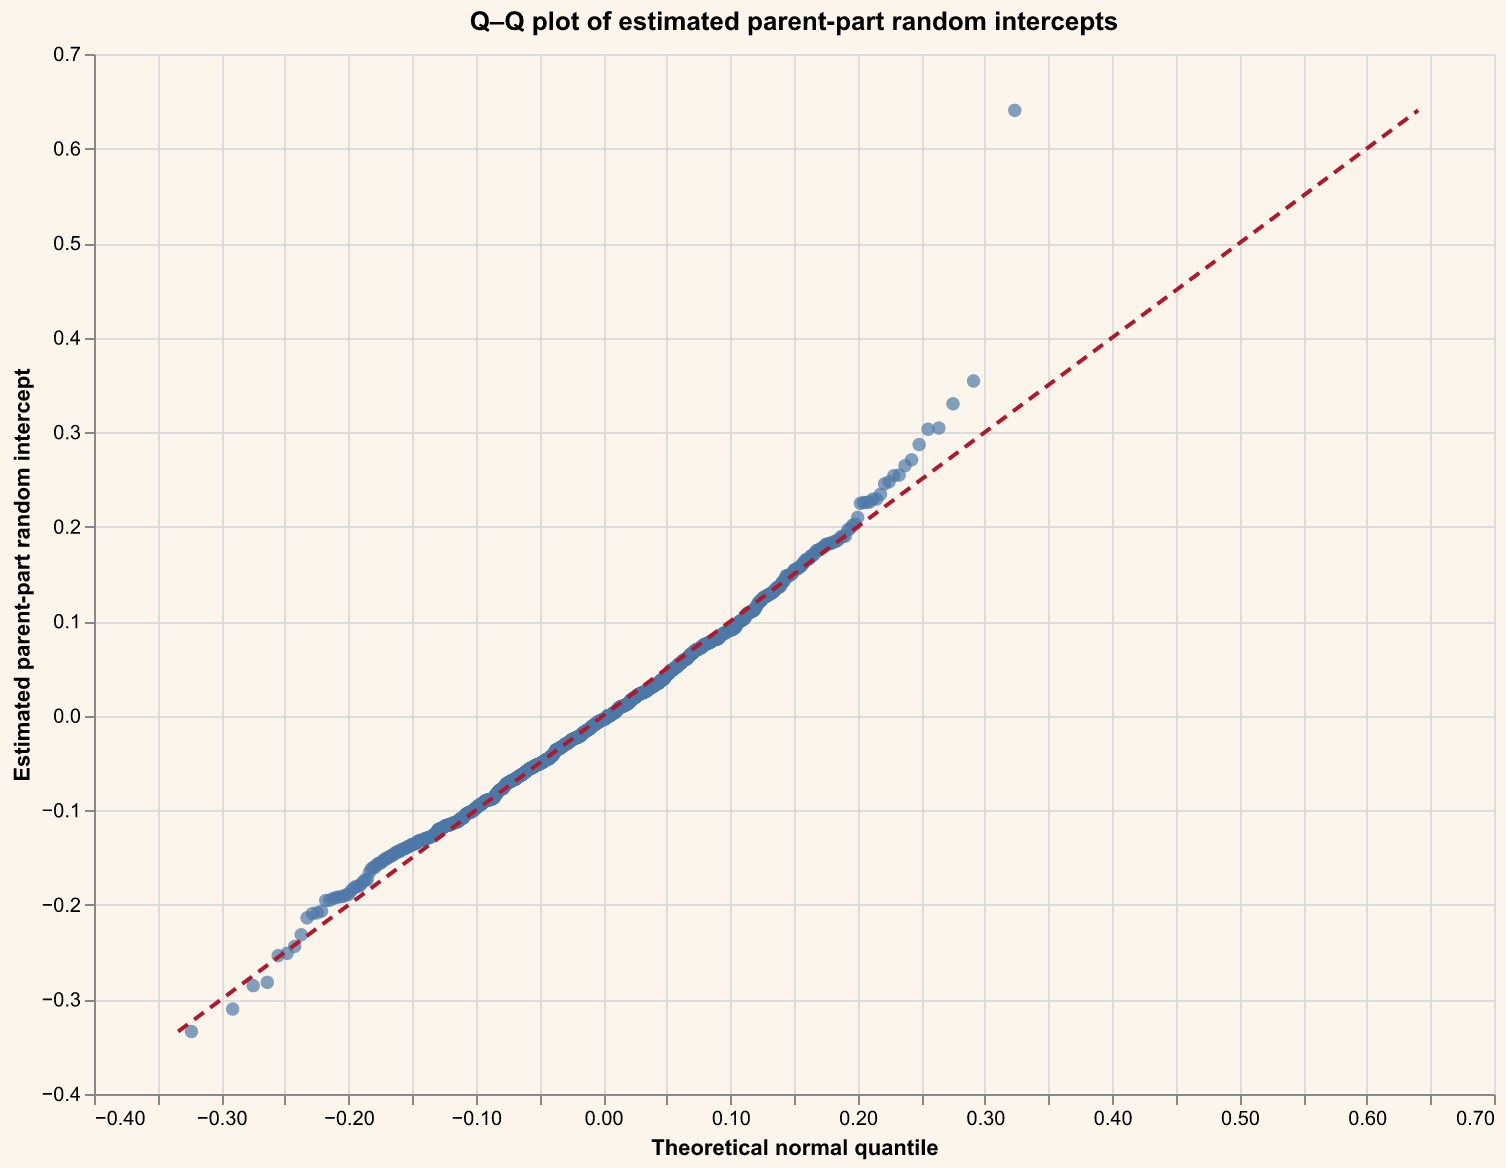
\includegraphics[keepaspectratio,alt={Parent-part Q--Q plot}]{outputs/charts/mc3-coh-pettype-final-model/parent_part_random_intercepts_qq.png}}

\pandocbounded{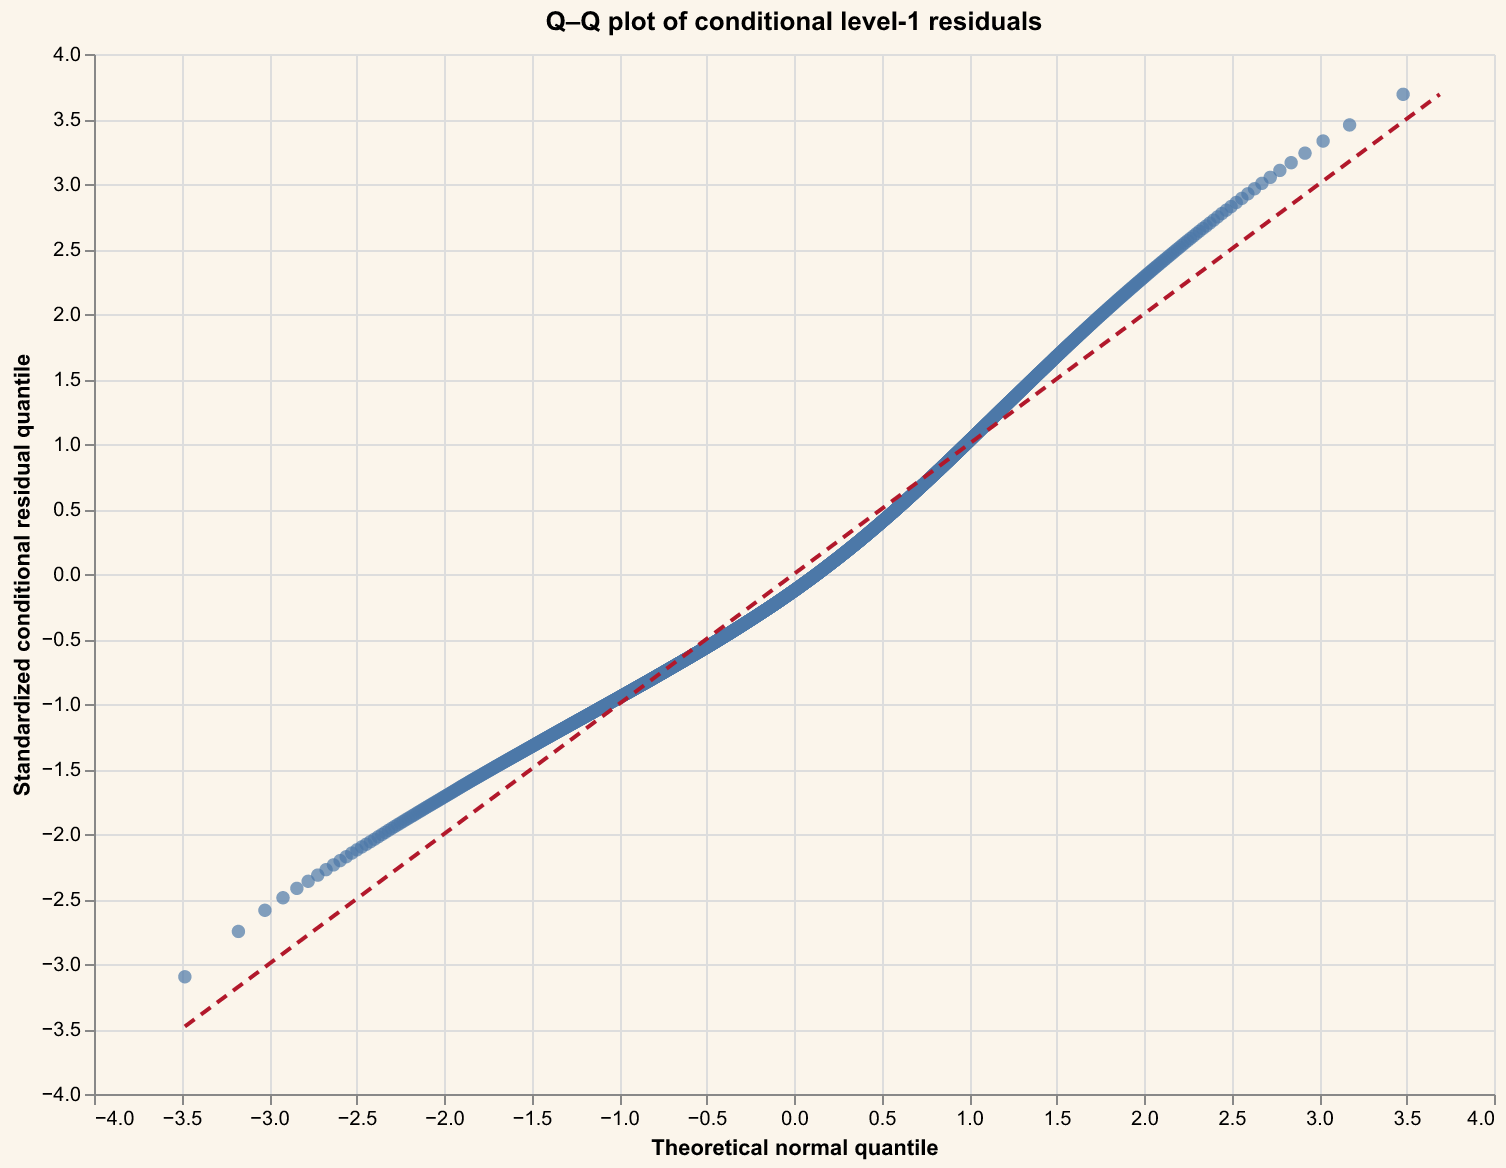
\includegraphics[keepaspectratio,alt={Residual Q--Q plot}]{outputs/charts/mc3-coh-pettype-final-model/conditional_residuals_qq.png}}

\pandocbounded{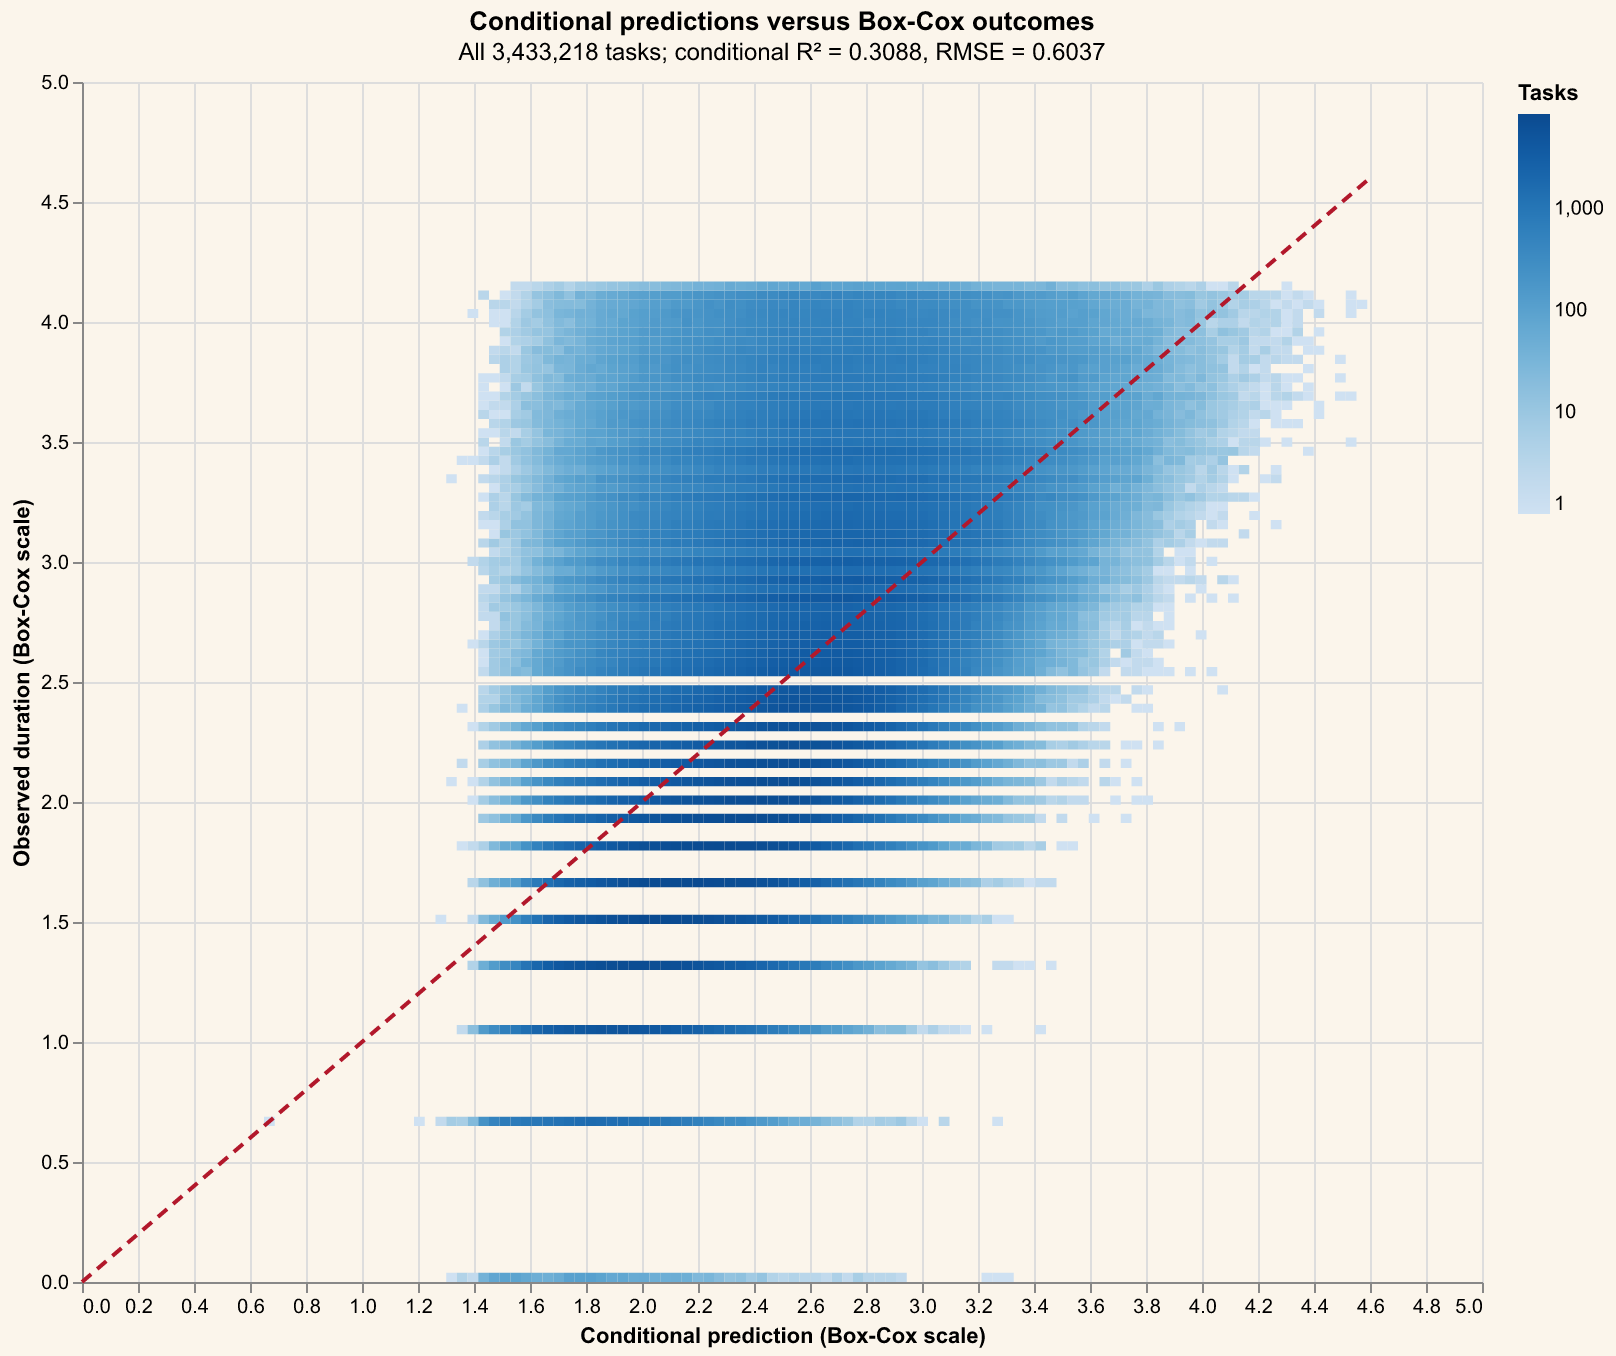
\includegraphics[keepaspectratio,alt={Predicted versus outcome}]{outputs/charts/mc3-coh-pettype-final-model/predicted_vs_boxcox_actual.png}}

%%% Local Variables:
%%% mode: LaTeX
%%% TeX-master: "../main"
%%% End:
\subsection{Estimating the Potential of Grouping Similar Tasks}

\Needspace{8\baselineskip}
\section{References}\label{references}
\begin{enumerate}[label={[\arabic*]},leftmargin=*]
\item \label{ref:grouping-similar-work}\emph{Would Grouping Similar Work Make Pharmacists Faster? What the data says}. Internal analysis. \url{https://chewyinc.atlassian.net/wiki/x/hYRyRQE}.
\item JD Wright. Cohort definitions and rationale. Internal conversation, undated; reproduced in the Appendix.
\item \label{ref:confounding}Wikipedia contributors. \emph{Confounding}. \url{https://en.wikipedia.org/wiki/Confounding}.
\item \label{ref:analysis-repository}\emph{RXP Pharmacist Task Grouping Analysis}. GitHub repository. \url{https://github.com/myunt1-chwy/rxp-pharmacist-task-grouping-analysis}.
\end{enumerate}
\end{document}
